\chapter[Transit timing variations of cool Kepler planets from Spitzer/IRAC analysis]{Transit timing variations of cool Kepler planets from Spitzer/IRAC analysis}
%\chaptermark{header title} %% if you want a different title in the headers
\label{TTVs}

% Define the location of your plots
\graphicspath{{./gfx/CoolKeplers/}}

% List all paper authors
\chauthors{Claire Baxter,
          Jean-Michel D\'esert,
          Daniel Fabrycky}

\chjournal{in preparation}


\begin{abstract}

Here we present the analysis of forty-eight transits of three multi-planet systems (Kepler-9, Kepler-18 and Kepler-32) and one circumbinary system (Kepler-16b) using \spitzerIRAC 3.6 and 4.5~$\mu$m photometric bandpasses. We analyze the lightcurves using our custom pipeline, which implements pixel level decorrelation to correct for the strong \spitzer systematics. We present the resulting transit parameters and transit times for each lightcurve. For the multi-planet systems we are able to constrain the transit times to around 8-minute precision for Kepler-9 and -18 and to around 40 minutes for Kepler-32. The flux from Kepler-16 is two orders of magnitude higher resulting in much better precision on the transit parameters, the transit times are constrained to the sub-minute level. We compare the transit times of the multi-planet systems to transit timing variation models which were calculated using \Kepler~data, and find that our times agree with the current predictions. However, the data demonstrates significant scatter compared to the \Kepler~data and so we cannot constrain the models any further. We compare the Kepler-16b \spitzer transit times to photodynamical predictions from the \Kepler~ data. We find that the transits occur significantly later than predicted. We, therefore, use the \spitzer transits in combination with the \Kepler~ transits to update the photodynamical model and report the new constraints on the orbital elements of the system.

\end{abstract}

%%%%%%%%%%%%%%%%%%%%%%%%%%%%%%%%%%%%%%%%%%%%%%%%%%

%%%%%%%%%%%%%%%%% BODY OF PAPER %%%%%%%%%%%%%%%%%%

\section{Introduction}

% Goals:
% - Test whether dynamical models from Kepler TTVs hold for these planets by measuring TTVs over different times than span by Kepler, and at different wavelength.
% - improve dynamical masses for these planets
% - look for additional signals that could be due to other planets
% - New model for Kepler-16

% Kepler mission
The \Kepler~mission \citep{Borucki2010} has provided us with a wealth of information on the exoplanet population. So far, there have been over 2800 planets discovered with \Kepler~and K2. Analysis of this population of planets has revealed that almost 50\% of stars in our galaxy are hosts to exoplanets, and that the most common type of planet are those with masses between the Earth and Neptune \citep{Batalha2013, Batalha2014, Fressin2013, Petigura2013a, Petigura2013b}. Out of these many newly discovered exoplanets resulting from the \Kepler~ mission, there are more than 700 multi-planet systems.

% multiplanet systems with Kepler
Prior to the launch of \Kepler, it was shown that numerically reproducing the dynamical interactions of multi-planet systems can provide constraints on the individual planet masses \citep{Holman2005, Agol2005}. Dynamical interactions in multi-planet systems cause deviations from Keplerian orbits resulting in variations in the orbital period which can be detected by measuring transit timing variations (TTVs). This technique was used to confirm the multi-planet system Kepler-9 and to measure the individual masses of the planets \citep{Holman2010}. TTV measurements with \Kepler~have yielded mass and eccentricity measurements for a significant number of planets, which is particularly useful for sub-Jovian planets where radial velocity signals are typically too small \citep{Jontof-Hutter2016,Hadden2017}. Mass and eccentricity constraints are crucial for understanding planetary formation and evolution.

% Spitzer high precision TRAPPIST
The Spitzer Space Telescope can also provide excellent precision on the transit times of multi-planetary systems \citep[e.g.,][]{Beichman2016, Gillon2017, Berardo2019}. \citet{Gillon2017} used the 4.5\um~ bandpass to continuously monitor the TRAPPIST-1 system, detecting 37 transits of the shortest period planet (TRAPPIST-1b) and 1 transit of the longest period planet (TRAPPIST-1h). They were able to measure the transit times of all seven Earth-size exoplanets to better than one minute precision.

% Multi-planet systems that we will look at
%Kepler-9
In this work, we study three multi-planet systems (Kepler-9, Kepler-18 and Kepler-32) and one circumbinary system (Kepler-16). Kepler-9 is a benchmark system consisting of two planets with relatively deep transits ($\sim$0.5\%) and one super-Earth orbiting a solar analog star with \Kepler-magnitude of 13.803 \citep{Holman2010}. \citet{Freudenthal2018} applies a photodynamical model to \Kepler~and ground-based observations of the Kepler-9 system to determine precise densities and predict the future dynamics of the system. Here, we use \spitzer/IRAC data to study the two innermost planets, Kepler-9b and Kepler-9c, in an attempt to compare the data to model predictions as well as study their atmospheres. These two planets have orbital periods near a 2:1 mean motion resonance, leading to TTV amplitudes on the order of one day \citep{Freudenthal2018}.

The second system we study is Kepler-18, another 3 planet system around another sun-like star, with a \Kepler-magnitude of 13.549. In this work, we study the two outermost low-density Neptune mass planets, Kepler-18c and Kepler-18b, which are accompanied by an inner super-Earth planet \citet{Cochran2011}. Kepler-18c and Kepler-18d also have orbital periods near a 2:1 mean-motion resonance, resulting in large TTV signals.

The third system is Kepler-32, a five-planet system around an M dwarf \citep{Muirhead2012} with \Kepler-magnitude of 15.801. Planet b and c have relatively short orbital periods in a 3:2 mean motion resonance, resulting in detectable TTV amplitudes in \Kepler. However, have relatively small transit depths ($\sim0.15$\%), which when combined with a faint star make their transits challenging.

The final planet we study is the circumbinary planet, Kepler-16b, which is on a 229 day orbital period around its two parent stars \citep{Doyle2011}. Kepler-16b now only transits star A, a 0.68 solar mass K-type star with \Kepler-magnitude 11.762. Here, we analyze two transits of Kepler-16b, at 3.6 and 4.5~\um~, two orbital periods apart. We aim to constrain the dynamics and planet mass using photo-dynamical models.
% Kepler-9 and 18 were originally too faint for RV measurements - not true
% Kepler-9
% Kepler-18
% Kepler-32

% Circumbinary system - Kepler-16b - photodynamical modelling

% This paper
This paper is organized as follows. We describe the observations in Section \ref{P4:sec:obs}, and the data analysis and lightcurve reduction in Section \ref{P4:sec:analysis}. We present the results on the transit times of each of our systems in Section \ref{P4:sec:results} and compare to predictions from TTV models in the case of the multi-planet systems and photo-dynamical model for Kepler-16b.

\section{Observations}
\label{P4:sec:obs}

Using \spitzer/Infrared Array Camera (IRAC), we observed a total of 46 transits at 3.6 and 4.5~\um~of three multi-planet Kepler systems: Kepler-9, Kepler-18 and Kepler-32. Additionally, we obtained two transit observations of the circumbinary planet Kepler-16b (one at 3.6~$\mu m$ and one at 4.5~$\mu m$). These transits were taken two orbital periods apart with the first (3.6~$\mu m$) observation taking place on UT 2013 September 23 and the second (4.5~$\mu m$) on UT 2014 December 18. Our observations are part of the survey program 90092 (PI Desert) and are thus taken during the Post Cryogenic Warm \spitzer/IRAC mission, meaning the data are in sub-array mode (32$\times$32 pixels) and only at 3.6 and 4.5~\um. Furthermore, all observations were taken in "peak-up" mode, which consists of a 30-minute throw-away observation allowing for accurate pointing and precise positioning of the target which reduces the ramp-up caused by the intrapixel sensitivity. Table \ref{P4:tab:obs} shows further details of our observations.


\longtab{
%\setlength{\tabcolsep}{3pt}
\begin{longtable}[h]{lllll}
  \caption{Details of the Spitzer Observations used in our survey analysis showing the UT date of observation, the duration of observation in hours and the program ID of each transit.}\\
\hline\hline
Target & $\lambda$ & UT Start Date &  Duration &  Program ID \\
& $\mu$ m & & Hours &  \\
\hline
\endfirsthead
\caption{continued.} \\
\hline\hline
Target & $\lambda$ & UT Start Date &  Duration &  Program ID \\
& $\mu$ m & & Hours &  \\

\hline
\endhead
\hline
\endfoot

Kepler-9b  &               3.6 &   2013 Jul 04 &         7.2 &       90092 \\
Kepler-9b  &               3.6 &   2013 Aug 31 &         7.2 &       90092 \\
Kepler-9b  &               3.6 &   2013 Dec 05 &         7.2 &       90092 \\
Kepler-9b  &               3.6 &   2014 Jan 12 &         7.2 &       90092 \\

Kepler-9b  &               4.5 &   2013 Aug 11 &         7.2 &       90092 \\
Kepler-9b  &               4.5 &   2013 Sep 19 &         7.2 &       90092 \\
Kepler-9b  &               4.5 &   2013 Dec 24 &         7.2 &       90092 \\
Kepler-9b  &               4.5 &   2014 Jul 24 &         7.2 &       90092 \\

Kepler-9c  &               3.6 &   2013 Jan 01 &         7.7 &       90092 \\
Kepler-9c  &               3.6 &   2013 Nov 09 &         7.7 &       90092 \\
Kepler-9c  &               3.6 &   2014 Jun 30 &         7.7 &       90092 \\
Kepler-9c  &               3.6 &   2014 Sep 16 &         7.7 &       90092 \\

Kepler-9c  &               4.5 &   2013 Oct 01 &         7.7 &       90092 \\
Kepler-9c  &               4.5 &   2013 Dec 18 &         7.7 &       90092 \\
Kepler-9c  &               4.5 &   2014 Aug 08 &         7.7 &       90092 \\
Kepler-9c  &               4.5 &   2014 Dec 02 &         7.7 &       90092 \\

Kepler-18c &               3.6 &   2012 Nov 28 &         6.3 &       90092 \\
Kepler-18c &               3.6 &   2012 Dec 13 &         6.3 &       90092 \\
Kepler-18c &               3.6 &   2013 Oct 22 &         6.3 &       90092 \\

Kepler-18c &               4.5 &   2013 Aug 15 &         6.3 &       90092 \\
Kepler-18c &               4.5 &   2013 Oct 07 &         6.3 &       90092 \\
Kepler-18c &               4.5 &   2014 Jan 07 &         6.3 &       90092 \\

Kepler-18d &               3.6 &   2012 Nov 22 &         6.3 &       90092 \\
Kepler-18d &               3.6 &   2013 Nov 13 &         6.3 &       90092 \\
Kepler-18d &               3.6 &   2013 Dec 28 &         6.3 &       90092 \\

Kepler-18d &               4.5 &   2013 Oct 15 &         6.3 &       90092 \\
Kepler-18d &               4.5 &   2013 Nov 28 &         6.3 &       90092 \\
Kepler-18d &               4.5 &   2014 Jan 27 &         6.3 &       90092 \\

Kepler-32b &               3.6 &   2013 Jul 29 &         4.5 &       90092 \\
Kepler-32b &               3.6 &   2013 Aug 04 &         4.5 &       90092 \\
Kepler-32b &               3.6 &   2013 Nov 18 &         4.5 &       90092 \\
Kepler-32b &               3.6 &   2014 Jan 05 &         4.5 &       90092 \\
Kepler-32b &               3.6 &   2014 Jan 22 &         4.5 &       90092 \\

Kepler-32b &               4.5 &   2013 Aug 22 &         4.5 &       90092 \\
Kepler-32b &               4.5 &   2013 Oct 20 &         4.5 &       90092 \\
Kepler-32b &               4.5 &   2013 Dec 06 &         4.5 &       90092 \\
Kepler-32b &               4.5 &   2014 Jan 16 &         4.5 &       90092 \\
Kepler-32b &               4.5 &   2014 Feb 09 &         4.5 &       90092 \\

Kepler-32c &               3.6 &   2013 Jul 26 &         4.5 &       90092 \\
Kepler-32c &               3.6 &   2013 Aug 04 &         4.5 &       90092 \\
Kepler-32c &               3.6 &   2013 Oct 22 &         4.5 &       90092 \\
Kepler-32c &               3.6 &   2013 Nov 08 &         4.5 &       90092 \\

Kepler-32c &               4.5 &   2013 Aug 13 &         4.5 &       90092 \\
Kepler-32c &               4.5 &   2013 Aug 30 &         4.5 &       90092 \\
Kepler-32c &               4.5 &   2013 Oct 30 &         4.5 &       90092 \\
Kepler-32c &               4.5 &   2013 Dec 22 &         4.5 &       90092 \\

Kepler-16b &               3.6 &   2013 Sep 23 &        13.6 &       90092 \\
Kepler-16b &               4.5 &   2014 Dec 18 &        13.6 &       90092 \\
\end{longtable}
}

\section{Data Analysis}
\label{P4:sec:analysis}
\subsection{\spitzer/IRAC lightcurve reduction}

We reduce the \spitzer/IRAC transit observations with our custom pipeline described fully in \citet{Baxter2021} which uses the pixel level decorrelation method from \citep{Deming2015}. The planets in \citet{Baxter2021} were selected for observation due to their high expected signal-to-noise ratio (S/N), these planets had an average K-magnitude of 10 resulting in high precision measurements on transit lightcurve parameters. The multi-planet Kepler systems in this work have a much lower expected S/N with an average K-mag of 12, two orders of magnitude fainter than the \citet{Baxter2021} sample. As an example, the average number of electrons detected in a 2-second exposure was $\sim$40,000 e- for all of the planets in \citet{Baxter2021}. This number determines the precision on each photometric data point due to photon counting statistics, and therefore determines the overall precision of the resulting parameters from fitting the transit lightcurve. For the multi-planet systems presented in this work, the average number of electrons detected in a 2 second exposure is $\sim$5,500 e-, resulting in large uncertainties and poorly constrained transit parameters. Due to the low signal-to-noise ratios (S/N) for all planets except Kepler-16b, we modified our approach in this work. For clarity, we recall the main steps of our pipeline and then note the changes for the low S/N planets.

In each of the Spitzer sub-array frames, we correct the dark current, flat field, and convert them to flux units before performing aperture photometry using a circular aperture around the calculated centroid position of the star. A full run of our original pipeline would create a grid of data reductions and finds the optimum methods and parameters for background subtraction, centroiding, and aperture photometry radius by means of a lowest reduced $\chi^2$ on the resulting lightcurves.

This method was followed for Kepler-16b, with details on the transit fitting below. However, for the other planets (Kepler-9, Kepler-18, and Kepler-32) we found that there was a very large spread in the fit parameters depending on the choice of pipeline parameters, the fit resulted in no transit being detected (transit depth of 0). We, therefore, studied all transit depths for every iteration of the pipeline and manually choose the optimum pipeline parameters (background subtraction, centroiding, and photometry radius). The criteria for the manual selection of the pipeline parameters were to have a non-zero and stable transit depth, i.e. small changes in pipeline parameters resulted in small changes in transit depths, then to keep the reduced $\chi^2$ as low as possible. Finally, we opted to use the same parameters for all AORs of each planet for consistency.

%We also calculate the midtimes of each photometric point from the UTC-based modified barycentric Julian date (MBJD) times in the file headers.

Uncertainties on the photometric points are calculated from photon noise and scaled up such that the reduced $\chi^2$ after an initial least-squares fit is equal to 1.

\subsection{\spitzer/IRAC lightcurve fitting}

The \spitzer/IRAC transit lightcurves are fit using the same method as in \citep{Baxter2021}. We fit the Spitzer systematics using Pixel Level Decorrelation \citep{Deming2015} and fit the transit using batman \citep{Kreidberg2015}. Due to the differences in S/N, we treat the multi-planet systems and Kepler-16 differently. However, all the tests performed and the method used to obtain the results on final parameters is a full Markov Chain Monte Carlo (MCMC) with 100 walkers, 500 throwaway burn-in steps, and 1000 production steps. We confirm convergence by looking at the autocorrelation time.

% Rp (Rj): 0.7885
% Rp_err (Rj): 0.00081
% a (AU): 0.140
% a_err (AU): 0.001
% R* (Rsol): 1.1
% R*_err (Rsol): 0.09
% Rp (R*): 0.0736824960382
% Rp_err (R*): 7.5691593901e-05
% a (R*): 27.3752839625
% a_err (R*): 5.05492095375
% b: 0.654
% b_err: 0.033
% inc (deg): 88.6310642411
% inc_err (deg): 10.582842764

\begin{table*}
\caption{Transit parameters and the corresponding reference for each of the Kepler planets. We show the semi-major axis ($a/R_s$), inclination, transit depth ($R_p/R_s$) and orbital period. Kepler-32 $a/R_s$ were calculated from $R_p(R_J)$ and a(AU). \label{P4:tab:transit}}
\centering
\begin{tabular}{llllll}
%\setlength{\tabcolsep}{3pt}
    \hline\hline
    System & $a/R_s$ & inclination & $R_p/R_s$ & Period & Ref. \\
     &  & $^{\circ}$ &  & days &  \\
    \hline
    Kepler-9b &  $31.3^{+1.1}_{-1.5}$  & $88.982^{+0.007}_{-0.005}$  &  $0.0776^{+0.0019}_{-0.0015}$ & 19.23891$\pm$0.00006 & 1 \\
    Kepler-9c &  $49.8^{+1.7}_{-2.6}$  & $89.188^{+0.005}_{-0.006}$  &  $0.0756^{+0.0018}_{-0.0014}$ & 38.9853$\pm$0.0003 & 1 \\
    Kepler-18c &  14.43$\pm$0.61  & 	87.68$\pm$0.22  &  0.04549$\pm$0.00055 & 7.64159$\pm$0.00003 & 2 \\
    Kepler-18d &  22.48$\pm$0.96  & 	88.07$\pm$0.10  &  0.05782$\pm$0.00069 & 	14.85888$\pm$0.00004 & 2 \\
    Kepler-32b* &  20.29$\pm$2.35 &  ... & 0.0389$\pm$0.0019 & 5.90124$\pm$0.00010	 & 3 \\
    Kepler-32c* &  36.52$\pm$7.60 &  ... & 0.0352$\pm$0.0033 & 8.7522$\pm$0.0003 & 3 \\
    Kepler-16b & ... & ... & ... & $228.776_{-0.037}^{+0.020}$ & 4 \\
    \hline
\end{tabular}
    \tablebib{\\
    (1)~\citet{Borsato2019};
    (2) \citet{Cochran2011};
    (3) \citet{Fabrycky2012};
    (4) \citet{Doyle2011};}
\end{table*}


\begin{table*}\setlength{\tabcolsep}{3pt}
\caption{\label{P4:tab:stars} Stellar parameters and the corresponding reference for each of the Kepler systems. We show the stellar effective temperature (\Teff), metallicity ([Fe/H]) and surface gravity (log(g)). Limb darkening co-efficients for a linear limb darkening law calculated from the 1D ATLAS code \citep{Sing2010} shown for 3.6 and 4.5\um.}
    \begin{tabular}{lllllll}
    \hline\hline
    System & \Teff & [Fe/H] & log(g) & 3.6\um~ ld & 4.5\um~ ld & Ref. \\
     & Kelvin & dex & $\rm log_{10}$(\cmss) & & &  \\
    \hline
    Kepler-9 &  5777 $\pm$ 61 & 0.12 $\pm$ 0.04  &  4.49 $\pm$ 0.09 & 0.202$\pm$0.004 & 0.175$\pm$0.003 & 1 \\
    Kepler-18 &  5345 $\pm$ 100 & 0.19 $\pm$ 0.06 & 4.31 $\pm$ 0.12 &  0.219$\pm$0.004 & 0.186$\pm$0.002 & 2 \\
    Kepler-32 & 3787 $\pm$ 117  & -0.1 $\pm$ 0.1  & 4.74 $\pm$ 0.08 & 0.165$\pm$0.017 & 0.157$\pm$0.010 & 3 \\
    Kepler-16 & 4450 $\pm$ 150 & -0.2 $\pm$0.2 & 4.6527 $\pm$ 0.0017 & 0.113$\pm$0.029 & 0.107$\pm$0.017 & 4 \\
    \hline
    \end{tabular}
    \tablebib{\\
(1)~\citet{Torres2011};
(2) \citet{Cochran2011};
(3) \citet{Dressing2013};
(4) \citet{Doyle2011} }
\end{table*}

%\subsection{Lightcurve fitting tests}

% Need to quantify all of this with numbers

\subsubsection{Obtaining the best fits of the multi-planet systems}

Due to the low signal-to-noise of the multi-planet systems, the final transit times are calculated by fixing the orbital distance ($a/R_s$), inclinations ($i$), and transit depths ($(R_p/R_s)^2$) to the literature values. These fixed values are displayed in Table \ref{P4:tab:transit}. We also fix the limb darkening to a linear law with parameters calculated from the 1D ATLAS code presented in \citep{Sing2010}. The stellar parameters use for this calculation are also displayed in Table \ref{P4:tab:stars}.

To determine the optimum transit times for the lightcurves, we performed several different tests when fitting the lightcurves. We compared each of our tests using the Bayesian Information Criterion (BIC) and by studying the precision on the resulting transit times. We aimed to have a uniform approach for each planet, so we calculated the average $\Delta$BIC and average improvement in timing precision over all the lightcurves for each planet to determine if the method had a statistically significant improvement on the fit for each planet.

% Which parameters to leave free?
The first test was determining which parameters we could leave free in the fits. When leaving the transit depth, semi-major axis, and inclination as free parameters the transit fits were often unconstrained, with the fits getting stuck at a transit depth of zero. We first tested fixing only the semi-major axis and the inclination (leaving $R_p/R_s$ free), the average $\Delta$BIC for all ten of the Kepler-9 lightcurves was 4, meaning that the difference between having $R_p/R_s$ fixed or free was not statistically significant. However, the precision retrieved on the final transit times of these fits was a factor of 1.5 smaller for $R_p/R_s$ fixed compared to when $R_p/R_s$ is free. For Kepler-32, leaving the transit depth free resulted in completely unconstrained transit parameters, so no information could be gained from these fits. We, therefore, opted to fix the transit parameters to literature values for studying the timing. However, leaving the transit depth free can provide us with information on the atmosphere so we show these results in Table \ref{P4:tab:keplerTDs} and Figure \ref{P4:fig:TD}.

% What about different sets of literature parameters
There are several different published values for each of our Kepler systems. For the Kepler-9 system we tested values from \citet{Holman2010} and \citet{Borsato2019}, we found that \citet{Holman2010} provided better fits and more precise measured transit times with a $\Delta$BIC of -32 compared to \citet{Borsato2019}. However, the more recent parameters from \citet{Borsato2019} resulted in improved precision on the final transit times (average of 8.3 minutes compared to 8.0 minutes), so these are the values presented in Section \ref{P4:sec:results}. For the Kepler-32 system, we tested transit parameters from \citet{Fabrycky2012} and \citet{Muirhead2012}. We found that the $\Delta$BIC between the two sets of parameters was marginally in favor of the \citet{Muirhead2012} parameters ($\Delta$BIC = -4) and that the results using these parameters had a 5-minute improvement on the precision of the transit times. Therefore, we use the \citet{Muirhead2012} parameters for the remainder of this work. For the Kepler-18 system, there was just one study providing the transit depth, inclination, and semi-major axis, so we used those transit parameters from \citet{Cochran2011}.

An additional source of error from the low signal to noise is increased scatter in the centroiding positions. We, therefore, tested fixing the centroiding to the mean over the whole lightcurve. We found that this induced more noise in the photometric lightcurve and resulted in worse fits with the average $\Delta$BIC for fixing the centroid compared to leaving the centroiding free was -0.5, -2.0, and -3.1 for Kepler-9, Kepler-18, and Kepler-32 respectively. This means that fixing the centroid made the fits marginally worse. It also had no significant improvement on the precision of the transit times. Furthermore, we also tried binning the data to improve the S/N, however,  we also found that this did not improve the precision of the times. % I no longer have the results from this test as I lost it with my old laptop.

% Testing priors
Finally, we tested Gaussian priors on some of our parameters. First, we tried a prior on the transit depth. We found that the average $\Delta$BIC from having priors was -5.3 with a slight decrease in the precision on the transit times. Secondly, we tried a prior on the transit depth, orbital distance, and inclination, which resulted in a $\Delta$BIC of -8.5.  Therefore, it was not helpful to have a prior on either the $(R_p/R_s)^2$ or on the $(R_p/R_s)^2$, $a/R_s$ and $i$.

In Section \ref{P4:sec:coolcompare} we compare the final transit times to TTV predictions using Kepler data. As a test, we also tried fixing the time with a prior on this parameter (as well as fixing semi-major axis, inclination, and transit depth as before) and compared the $\Delta$BIC. We found that the $\Delta$BIC was -16.6, meaning that the fits are better when there is no prior on the time.

\subsubsection{Obtaining the best fits of the Kepler-16 system}

Kepler-16 is of similar magnitude ($m_{_{\rm \litl Ks}}=8.996\pm0.022$) to the planets presented in \citet{Baxter2021}, which allows us to use the same data reduction method. Using this method \citep[outlined in ][]{Baxter2021}, we determined that the optimum parameters for extracting the light curve were to centroid using a Moffat function, background subtract using a circular annulus centered on the star with a minimum radius of 6 and a maximum radius of 10, and to perform aperture photometry with a radius of 2.5 pixels around the star. We also found that the best fit for correcting the initial ramp-up was to remove the first 15 minutes of the 4.5~\um~ lightcurve. However, the 3.6~\um~ is more complicated since the ingress falls at the very beginning of the observation. We tested cutting the beginning of the lightcurve at 2-minute intervals but determined that the best fits were obtained by using all of the data, therefore, no cut was performed at the beginning of the 3.6~\um~lightcurve.

Furthermore, the high S/N of the Kepler-16b lightcurves allows us to accurately constrain the transit parameters. Therefore, in our fits we left the transit depth (($R_p/R_s)^2$), the orbital distance ($a/R_s$), the inclination ($i$), the transit time ($T_0$) and the systematic parameters all free. We fixed the orbital period to $228.776_{-0.037}^{+0.020}$ \citep{Doyle2011} and the eccentricity and angle of periastron passage to 0. We also tried fixing the eccentricity and angle of periastron passage to 0.0069 and 318.0, respectively, however, we found that this had a negligible effect on the final parameters, with every parameter in every channel being consistent to less than 0.37$\sigma$
% Run a test on the eccentricity and angle of periastron passage to see if this affects the ingress/egress

We also fix the parameters of a linear limb darkening law with limb darkening parameters calculated from the 1D ATLAS code presented in \citep{Sing2010}, these parameters and the stellar parameters use for this calculation are displayed in Table \ref{P4:tab:stars}.

\subsection{TTV predictions of the multi-planet systems}
\label{P4:sec:TTVpred}

% first the kepler data (maybe these are subsubsections?)
Here we describe the dynamical analysis of the Kepler data, which allowed us to schedule the Spitzer observations originally, as well as determine how the knowledge of the dynamics of the systems are enhanced by the new data.

For the single-star systems (Kepler-9, 18, and 32), transit times are derived from the simple-aperture photometry provided on the Mikulski Archive for Space Telescopes (MAST) data portal. The transits are initially masked, and the coefficients to the first five contending basis vectors are adjusted to best-fit each quarter of data, after which that baseline is subtracted. A common shape model is assumed for all transits, based on the rectilinear motion of a planet across a linear limb-darkened star within the code of \cite{Mandel2002}, times a quadratic baseline covering 3 transits, centered on an initial guess for the transit time. Each transit mid-time is adjusted, simultaneous with the parameters of the shape model by $\chi^2$ minimization, via the Levenberg-Marquardt algorithm, resulting in the data presented in Table \ref{P4:tab:keplerTs}.

% the the model
An N-body model, described by \citep{Fabrycky2010}, is run with DEMCMC to determine the error bars on orbital elements and masses. A subset of the resulting chain is propagated forward in time to the Spitzer observations, yielding a posterior for the times of transits. These values may be used as priors on the photometric fits, or they may simply be compared with the results of the Spitzer analysis. If the latter, a difference between the Kepler predictions and the Spitzer observations may be interpreted as missing components of the model, e.g. previously unknown perturbers.

\begin{table*}
\caption{Transit times in units of $\rm BJD_{TDB}$ - 2454900 measured with \Kepler~ for each of the multi-planet systems (Kepler 9, 18 and 32). Showing the first ten transits for each system, full data from the 4 year mission available electronically.}
\label{P4:tab:keplerTs}
    \begin{tabular}{lllllll}
      \hline\hline
      Kepler-9b &  Kepler-9c & Kepler-18c    \\
      \hline
       77.249373 $\pm$    0.000796 &   69.306589 $\pm$    0.001039 &  60.769501 $\pm$     0.001044    \\
       96.483689 $\pm$    0.000700 &  108.331810 $\pm$    0.001211 &  68.407929 $\pm$     0.001051    \\
      134.955219 $\pm$    0.000674 &  147.336255 $\pm$    0.001194 &  76.050937 $\pm$     0.001472    \\
      154.191546 $\pm$    0.000534 &  186.313195 $\pm$    0.001747 &  83.692455 $\pm$     0.001207    \\
      173.434560 $\pm$    0.000907 &  225.263861 $\pm$    0.000786 &  91.334704 $\pm$     0.001689    \\
      211.926312 $\pm$    0.000935 &  264.184471 $\pm$    0.001091 & 106.611826 $\pm$     0.001600    \\
      231.172271 $\pm$    0.000391 &  303.071831 $\pm$    0.001059 & 114.255395 $\pm$     0.001632    \\
      250.430550 $\pm$    0.000580 &  341.930204 $\pm$    0.001084 & 121.896125 $\pm$     0.001352    \\
      269.681775 $\pm$    0.000945 &  380.765554 $\pm$    0.000807 & 129.536438 $\pm$     0.001212    \\
      288.946342 $\pm$    0.000416 &  419.578253 $\pm$    0.000940 & 137.178077 $\pm$     0.001146    \\
      ... & ... & ... \\
      \\
      \hline\hline
      Kepler-18d &  Kepler-32b &  Kepler-32c \\
      \hline
      61.151516 $\pm$     0.000892 &   68.993086 $\pm$     0.006401 &   68.630187 $\pm$     0.009214 \\
      76.011567 $\pm$     0.000973 &   74.909074 $\pm$     0.004925 &   77.395221 $\pm$     0.010078 \\
      90.870969 $\pm$     0.000741 &   80.791214 $\pm$     0.008591 &  103.646223 $\pm$     0.010308 \\
      105.730819 $\pm$     0.000787 &   86.685556 $\pm$     0.009716 &  112.378658 $\pm$     0.013648 \\
      120.593162 $\pm$     0.001387 &   92.606325 $\pm$     0.006081 &  121.129198 $\pm$     0.009362 \\
      135.449711 $\pm$     0.000847 &  104.400104 $\pm$     0.008117 &  129.887968 $\pm$     0.010674 \\
      150.308328 $\pm$     0.000845 &  110.293412 $\pm$     0.006943 &  138.628310 $\pm$     0.006710 \\
      165.169560 $\pm$     0.000826 &  122.101891 $\pm$     0.006287 &  147.378278 $\pm$     0.008525 \\
      180.024765 $\pm$     0.002150 &  128.019136 $\pm$     0.004992 &  156.159973 $\pm$     0.009048 \\
      194.885133 $\pm$     0.000999 &  133.907354 $\pm$     0.005382 &  164.889254 $\pm$     0.009799 \\
      ... & ... & ... \\
      \hline
    \end{tabular}
\end{table*}


\subsection{Kepler-16b photodynamical model}

% then describe the model
A photodynamical model was developed in the Ph.D. thesis of S. Mills, where it was applied to both resonant system \citep{Mills2016} and planets around binary systems \citep{Welsh2015}. This model was applied to the long-cadence photometric data of Kepler-16. The data were prepared by masking the transit times, then de-trending by fitting a cubic polynomial, within a sliding 2-day wide window.

Starting with orbital elements that were optimized to the first 600 days of Kepler photometry \citep{Doyle2011}, a differential-evolution Markov Chain Monte Carlo \citep[DEMCMC;][]{TerBraak2005} fit was performed, including the radial velocity values. A run of 40 walkers for 4300 generations yielded a best-fit, which was propagated forward to make photometric predictions for the Spitzer data.

We found that these best-fit times were considerably early ($14$~min) for the second transit, showing that actually including Spitzer data in the fit would give better constraints on the orbits. We ran the DEMCMC fit with the Kepler and Spitzer data combined. A common limb darkening was used, which allows the fit to correctly adjust to the timing of the Spitzer data, but not the shape. The parameters of the quadratic limb darkening for the Kepler bandpass are 0.652201 and 0.017569 for the 1st and 2nd order coefficients. For display purposes, we have plotted this model with Kepler limb-darkening, for the Spitzer transit we can optimize the limb darkening as a post-processing step.

\section{Results}
\label{P4:sec:results}

\subsection{Transit times for the multi-planet systems}

The final photometric lightcurves of Kepler-9b and -9c, Kepler-18c and -18d and Kepler-32b and -32c are shown in Figure \ref{P4:fig:normlcK9}. The measured transit times for each lightcurve are displayed in Table \ref{P4:tab:results}. In this table, we also show the error on the transit time in minutes as well as the fraction that the lightcurve was above photon noise. In terms of errors on the transit time, the Kepler-9 and Kepler-18 transit times are significantly better constrained compared with the Kepler-32 transit times. All three stars are of a similar magnitude and we obtain a similar level of precision in terms of the percentage of photon noise for all of the transits. So the lower precision on the transit times of the Kepler-32 planets is likely due to them having a significantly smaller transit depth signal due to the smaller relative size of the planet.

In these transit time results, there are three AORs of Kepler-9 and Kepler-18 (r47029248, r47060992, r47056128) that have very large errors on the transit times. Each of these three transits either has a poor correction of the instrumental systematics or they are almost partial transits, i.e. the ingress or egress falls close to the beginning or end of observation respectively. This can result in the transit timing having very large errors are the shape of the transit is not properly constrained.

Additionally, in Appendix Table \ref{P4:tab:keplerTDs} and Figure \ref{P4:fig:TD} we also list and plot the results from the fits where the transit depth was also a free parameter of the lightcurves of Kepler-9 and Kepler-18. We calculate the weighted mean of these transit depths for each bandpass following the method outlined in \citet{Ingalls2016}. The individual transit depths exhibit significant scatter compared to each other and the weighted means do not demonstrate a significant atmospheric signal between 3.6 and 4.5\um. We calculate the normalized transit depth difference used in \citet{Baxter2021} ($(\delta_{ch2} - \delta_{ch1})/\delta_{ch1}$) and find that all 4 planets are within 1$\sigma$ of zero. This could either indicate that these planets are cloudy or that we do not have significant precision to measure the atmospheric signal.


\longtab{

%\setlength{\tabcolsep}{3pt}

\begin{longtable}[h]{lllllll}

\caption{\label{P4:tab:results}Table of measured transit times (in BJD\textsubscript{UTC}) for each of the six Kepler planets. We also show the uncertainty on the time converted to minutes, the fraction above photon noise and the deviation from the TTV predictions.}\\
\hline\hline
Planet & AOR & $\lambda$ &  T0 &   $\sigma_{\rm T0}$ & Photon noise & O-C\\
& & $\mu$m & $\rm BJD_{UTC}$ & Minutes &  & N$\sigma$ \\
\hline
\endfirsthead
\caption{continued.} \\
\hline\hline
Planet & AOR & $\lambda$ &  T0 &   $\sigma_{\rm T0}$ & Photon noise & O-C\\
& & $\mu$m & $\rm BJD_{UTC}$ & Minutes &  & N$\sigma$ \\
\hline
\endhead
\hline
\endfoot
Kepler9b  &  r47043072 &     3.6 & 2456670.630 $\pm$ 0.003 &       3.9 & 2.8 &  0.66 \\
Kepler9b  &  r47043584 &     3.6 & 2456632.131 $\pm$ 0.003 &       3.7 & 2.9 &  2.63 \\
Kepler9b  &  r47044352 &     3.6 & 2456535.881 $\pm$ 0.004 &       5.5 & 3.2 & -8.47 \\
Kepler9b  &  r47044608 &     3.6 & 2456478.207 $\pm$ 0.003 &       4.6 & 2.9 & -3.08 \\
Kepler9b  &  r47054336 &     4.5 & 2456863.317 $\pm$ 0.003 &       4.1 & 2.9 & -0.66 \\
Kepler9b  &  r47054592 &     4.5 & 2456651.375 $\pm$ 0.003 &       4.0 & 2.6 &  1.66 \\
Kepler9b  &  r47054848 &     4.5 & 2456555.152 $\pm$ 0.004 &       5.1 & 2.7 &  0.04 \\
Kepler9b  &  r47055104 &     4.5 & 2456516.679 $\pm$ 0.003 &       4.4 & 2.6 & -0.57 \\
Kepler9c  &  r47029248 &     4.5 & 2456994.481 $\pm$ 0.010 &      14.2 & 6.1 & -1.50 \\
Kepler9c  &  r47061760 &     3.6 & 2456293.779 $\pm$ 0.003 &       4.6 & 2.8 &  3.63 \\
Kepler9c  &  r47061504 &     3.6 & 2456606.048 $\pm$ 0.003 &       4.4 & 2.8 & -3.98 \\
Kepler9c  &  r47060992 &     3.6 & 2456839.407 $\pm$ 0.033 &      47.5 & 2.9 &  2.44 \\
Kepler9c  &  r47060480 &     3.6 & 2456916.899 $\pm$ 0.004 &       5.3 & 3.8 & -3.94 \\
Kepler9c  &  r47030016 &     4.5 & 2456567.072 $\pm$ 0.004 &       5.1 & 2.7 & -2.58 \\
Kepler9c  &  r47029760 &     4.5 & 2456645.005 $\pm$ 0.005 &       7.2 & 2.7 & -1.13 \\
Kepler9c  &  r47029504 &     4.5 & 2456878.118 $\pm$ 0.003 &       4.4 & 3.1 & -2.09 \\
Kepler18c &  r46858496 &     3.6 & 2456259.836 $\pm$ 0.005 &       7.8 & 2.4 & -0.06 \\
Kepler18c &  r47045376 &     3.6 & 2456275.121 $\pm$ 0.005 &       7.4 & 2.3 &  0.33 \\
Kepler18c &  r47045120 &     3.6 & 2456588.422 $\pm$ 0.005 &       7.0 & 2.3 &  0.33 \\
Kepler18c &  r47056640 &     4.5 & 2456519.646 $\pm$ 0.004 &       6.2 & 2.0 & -0.95 \\
Kepler18c &  r47056384 &     4.5 & 2456573.156 $\pm$ 0.004 &       6.0 & 2.0 &  4.18 \\
Kepler18c &  r47056128 &     4.5 & 2456664.876 $\pm$ 0.066 &      94.5 & 2.0 &  0.67 \\
Kepler18d &  r46867456 &     3.6 & 2456253.880 $\pm$ 0.003 &       4.1 & 2.3 &  1.04 \\
Kepler18d &  r47063808 &     3.6 & 2456610.491 $\pm$ 0.002 &       2.5 & 2.2 & -2.32 \\
Kepler18d &  r47063552 &     3.6 & 2456655.057 $\pm$ 0.003 &       4.8 & 2.1 & -4.97 \\
Kepler18d &  r47033600 &     4.5 & 2456580.774 $\pm$ 0.005 &       6.9 & 2.0 & -0.14 \\
Kepler18d &  r47033344 &     4.5 & 2456625.344 $\pm$ 0.003 &       4.0 & 2.1 & -3.68 \\
Kepler18d &  r47033088 &     4.5 & 2456684.785 $\pm$ 0.003 &       3.8 & 2.1 & -2.10 \\
Kepler32b &  r47032320 &     3.6 & 2456503.279 $\pm$ 0.040 &      57.4 & 3.5 & -1.23 \\
Kepler32b &  r47031808 &     3.6 & 2456509.223 $\pm$ 0.006 &       8.3 & 3.8 & -0.99 \\
Kepler32b &  r47031296 &     3.6 & 2456615.503 $\pm$ 0.058 &      83.2 & 3.0 &  0.77 \\
Kepler32b &  r47030528 &     3.6 & 2456662.613 $\pm$ 0.028 &      40.0 & 3.1 & -2.05 \\
Kepler32b &  r47030272 &     3.6 & 2456680.310 $\pm$ 0.027 &      38.2 & 3.8 & -2.37 \\
Kepler32b &  r47042560 &     4.5 & 2456526.904 $\pm$ 0.033 &      47.8 & 2.9 & -0.89 \\
Kepler32b &  r47042048 &     4.5 & 2456585.975 $\pm$ 0.030 &      43.8 & 2.7 &  0.78 \\
Kepler32b &  r47041536 &     4.5 & 2456633.170 $\pm$ 0.007 &      10.4 & 2.7 &  0.87 \\
Kepler32b &  r47040768 &     4.5 & 2456674.474 $\pm$ 0.017 &      23.9 & 2.8 &  0.11 \\
Kepler32b &  r47040256 &     4.5 & 2456698.079 $\pm$ 0.033 &      47.8 & 2.9 &  0.14 \\
Kepler32c &  r47048192 &     3.6 & 2456500.226 $\pm$ 0.012 &      16.6 & 3.4 & -2.15 \\
Kepler32c &  r47047936 &     3.6 & 2456509.010 $\pm$ 0.007 &       9.5 & 3.9 &  1.00 \\
Kepler32c &  r47047680 &     3.6 & 2456587.767 $\pm$ 0.016 &      23.5 & 3.3 &  0.10 \\
Kepler32c &  r47047424 &     3.6 & 2456605.238 $\pm$ 0.026 &      37.7 & 3.0 & -1.11 \\
Kepler32c &  r47059968 &     4.5 & 2456517.709 $\pm$ 0.038 &      54.0 & 2.9 & -1.24 \\
Kepler32c &  r47059712 &     4.5 & 2456535.252 $\pm$ 0.021 &      29.6 & 2.9 & -0.31 \\
Kepler32c &  r47059456 &     4.5 & 2456596.483 $\pm$ 0.049 &      71.2 & 2.8 & -0.69 \\
Kepler32c &  r47059200 &     4.5 & 2456649.088 $\pm$ 0.047 &      67.5 & 2.7 &  1.33 \\
\end{longtable}
}


\subsection{Comparing multi-planet system transit times to predictions}
\label{P4:sec:coolcompare}

In Figure \ref{P4:fig:TTVs} we compare the \spitzer~ transit times to predictions from the Kepler data, described in Section \ref{P4:sec:TTVpred}. We calculate the Observed - Calculated times by fitting a straight line to the Kepler observations ($O_E = P*E + T_0$) where $O_E$ are the observed times, $P$ is the period, $T_0$ is the ephemeris and $E$ is the integer transit number ($E$ = 0 is set to the closest value to $T_0$). This yields values for $P$ and $T_0$ which can be propagated to create $C_E$, a list of calculated transit times. These times are then subtracted from the observed \Kepler~ times ($O_E$), as well as the model prediction and the \spitzer~ times.

\begin{sidewaysfigure}
    \centering
    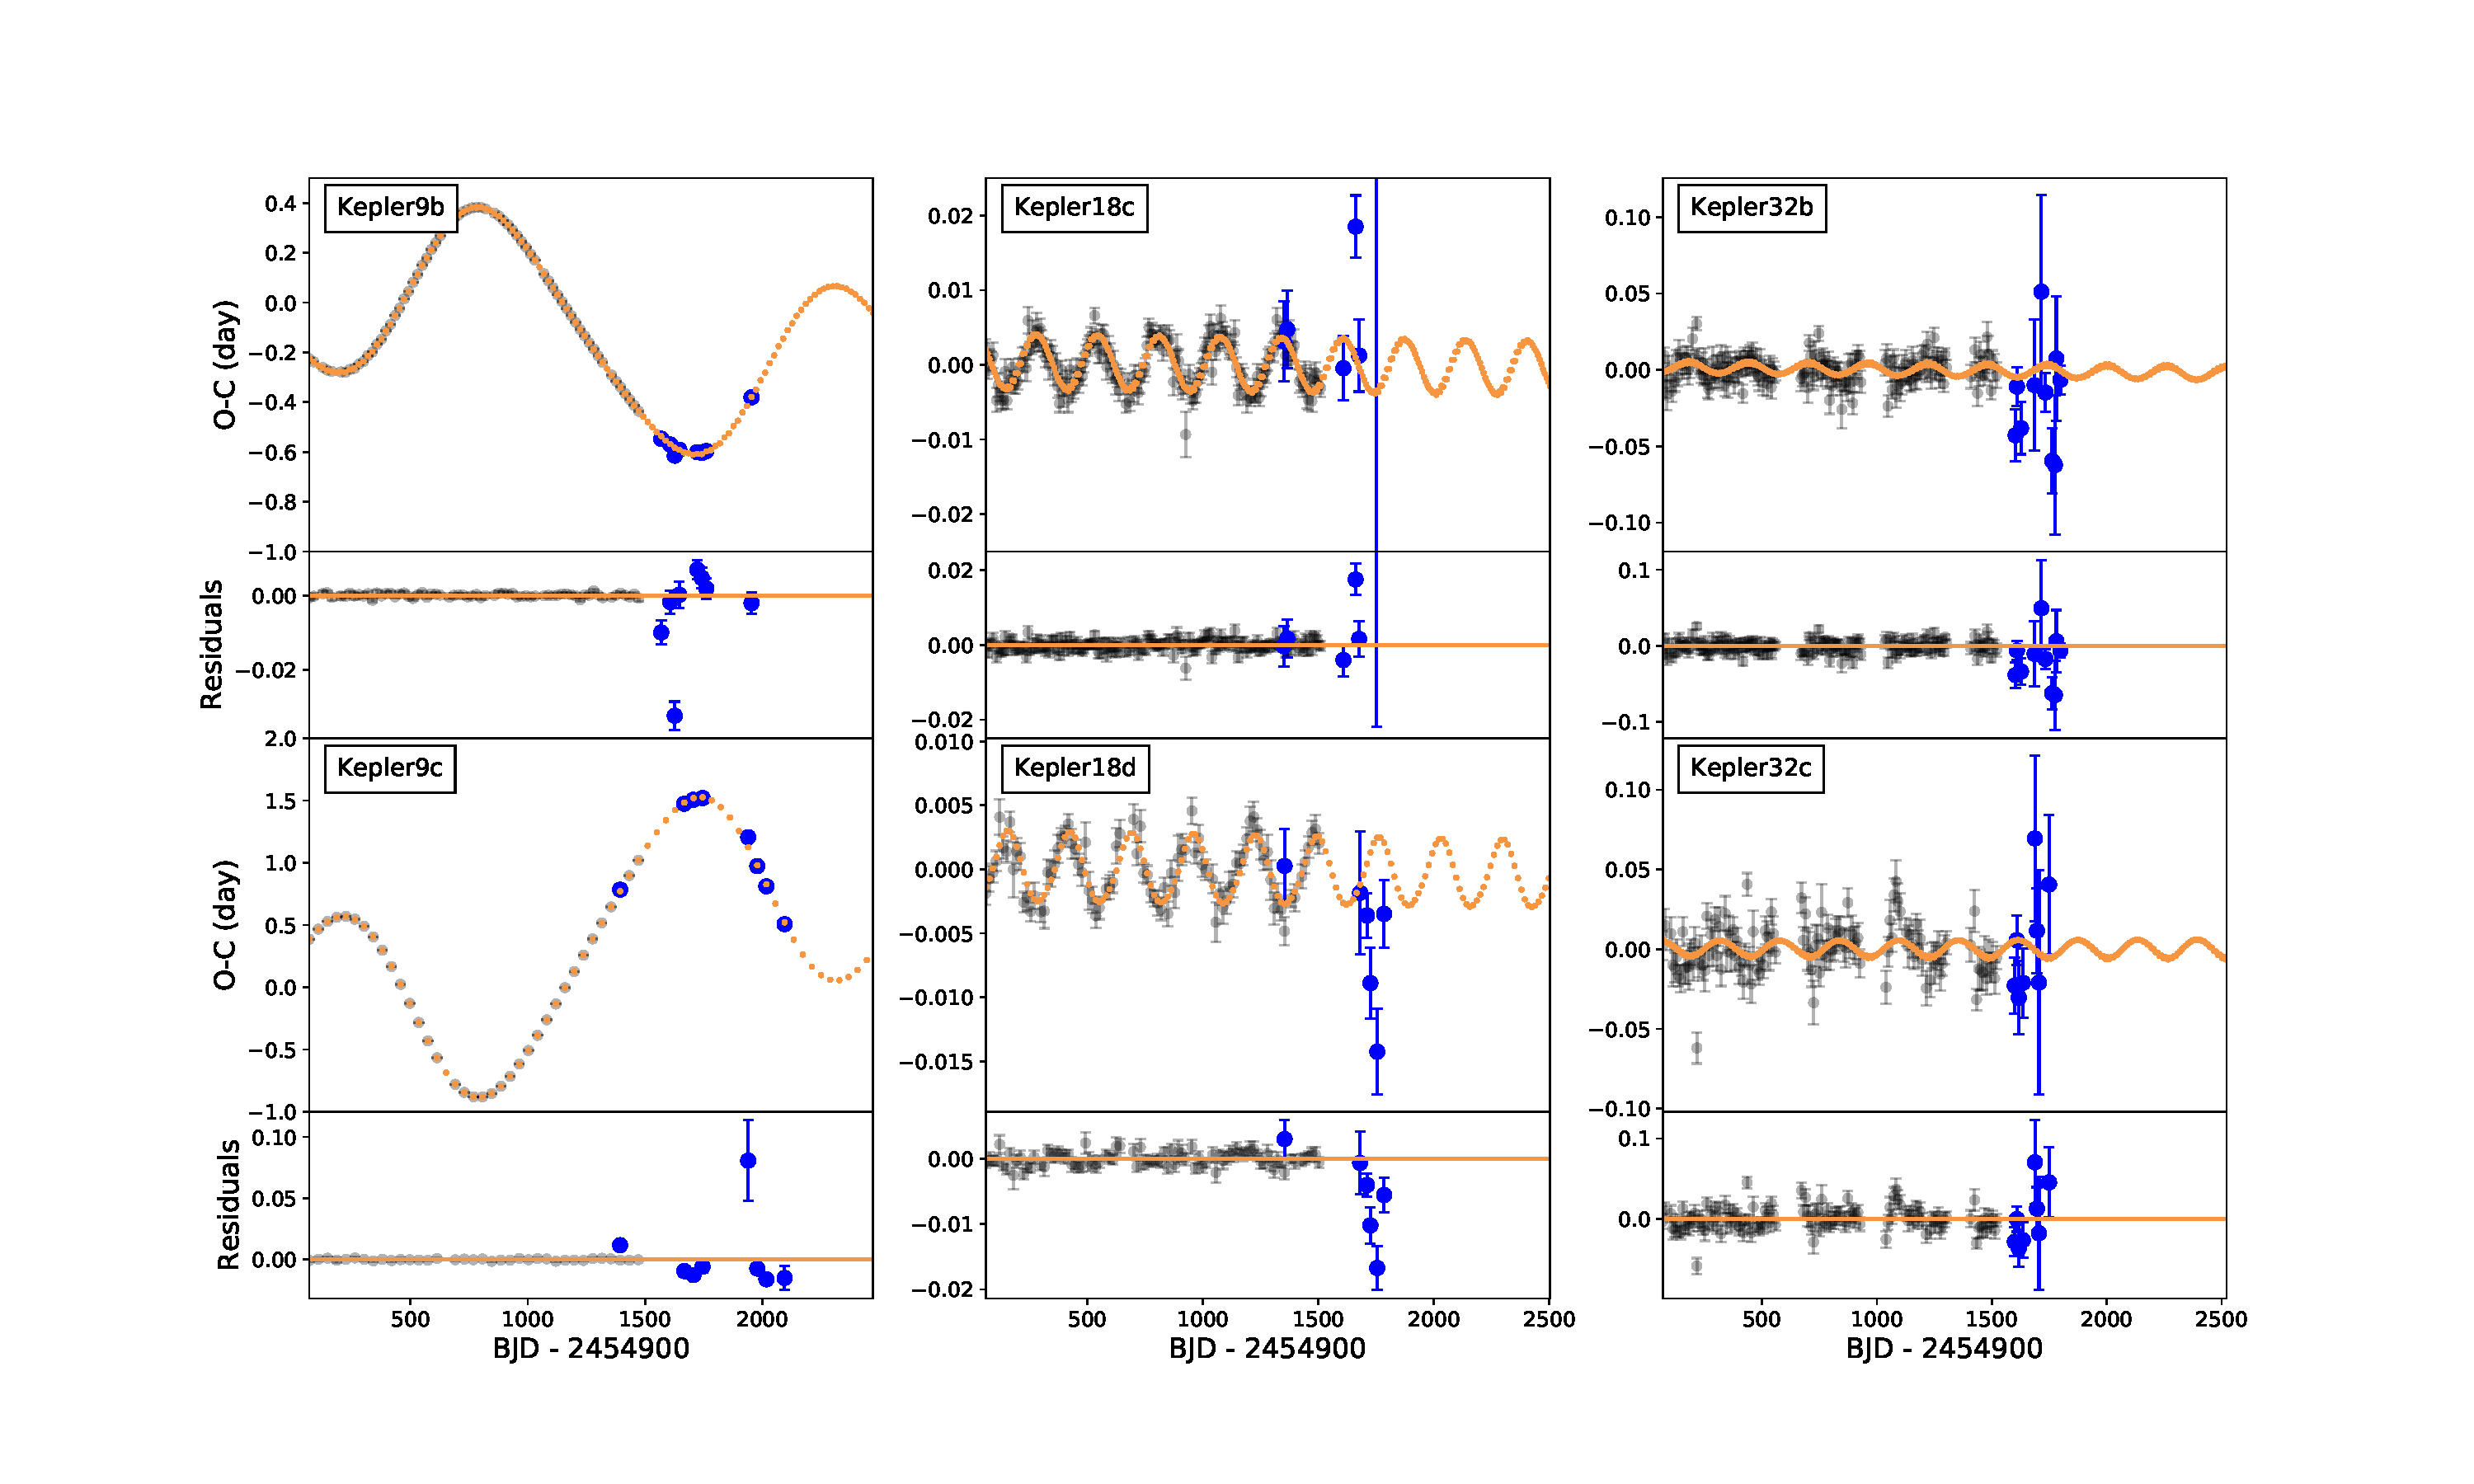
\includegraphics[trim=110 70 110 90, clip, width = \textwidth]{TTVs.pdf}
    \caption{First and third rows: The O-C diagrams of transit times and predictions from the \Kepler data and the newly analyzed \spitzer~ data for Kepler-9b, Kepler-9c, Kepler-18c, Kepler-18d, Kepler-32b and Kepler-32c. Calculated times are from a linear ephemeris fit to the Kepler data. Second and fourth rows: The residuals for the O-C diagrams.}
    \label{P4:fig:TTVs}
\end{sidewaysfigure}

In Table \ref{P4:tab:results} we show the number of standard deviations between the measured transit times and the TTV predictions. In absolute value, these planets are on average not significantly deviating from the TTV predictions (average N$\sigma$ is 1.7$\sigma$) and are thus not constraining to the TTV models.

\subsection{Kepler-16b lightcurves and transit parameters}

The raw transit lightcurves, corrected lightcurves, best-fit models, residuals, and root mean squared (RMS) vs bin size of Kepler-16b are shown in Figure \ref{P4:fig:k16blc} for channel 1 and channel 2 respectively. Before scaling up the uncertainties, we found that the 3.6~$\mu m$ and 4.5~$\mu m$ errors were 1.3 and 1.24 times photon noise respectively. This is standard for warm Spitzer/IRAC lightcurves, e.g. see \citet{Baxter2021}.

The RMS vs bin size plot demonstrates how well the correlated noise is corrected by comparing with the Poisson expectation ($\sqrt{N}$). For channel 1 there is a deviation from Poisson, indicating there is some red noise remaining in the lightcurve, this can also be seen in the residuals and is likely due to the extremely short-out-of-transit baseline before the transit. We tested cutting different amounts of time in 2-minute intervals from the beginning of the lightcurve. We found that there was a degeneracy with the amount of time cut off and the transit parameters ($R_p/R_s$, $a/R_s$ and inclination). In particular, we noted that the more time we cut off the smaller the measured transit depth. In a typical Spitzer observation, failing to remove the ramp-up at the beginning of the lightcurve has the effect of reducing the measured transit depth. Therefore, we should see a positive correlation with an increasing amount of time cut off at the beginning of the observation and the measured transit depth. However, in our case, we see that cutting the beginning of the observation also reduces the transit depth. We conclude that this is because we are cutting off too much of the ingress, which would also reduce the transit depth, and so we opted to keep all of the data. In Appendix Figures \ref{P4:fig:K16b_corner_ch1} and \ref{P4:fig:K16b_corner_ch2} we show the corner plots resulting from the MCMC calculation of Kepler-16b. Due to the 3.6\um~lightcurve observation starting very close to ingress, the corner plot shows that there is also a slight degeneracy with the transit depth and the temporal ramp parameter ($g$). In the end, this results in the uncertainty on the transit depth (\rprss) at 3.6\um~ being larger.

Additionally, both corner plots demonstrate the degeneracy between the semi-major axis and inclination, which is a common degeneracy when fitting the transit. Typically, we would fix these parameters either to literature values or to the mean of the two Spitzer transit lightcurves (e.g., see \citet{Baxter2021}). However, Kepler-16b has undergone significant precession over the duration between the two observations (two orbital periods) and so these parameters need to be left free in our fits. We are therefore able to use this information to constrain the photometric models.

In Table \ref{P4:tab:spitzerresults} we display the resulting best fit transit parameters for 3.6 and 4.5 $\mu$m. We measure the exquisite precision on the transit time of both transits, with uncertainties of 17 and 22 seconds for 3.6 and 4.5 $\mu$m respectively.

\begin{figure}
    \centering
    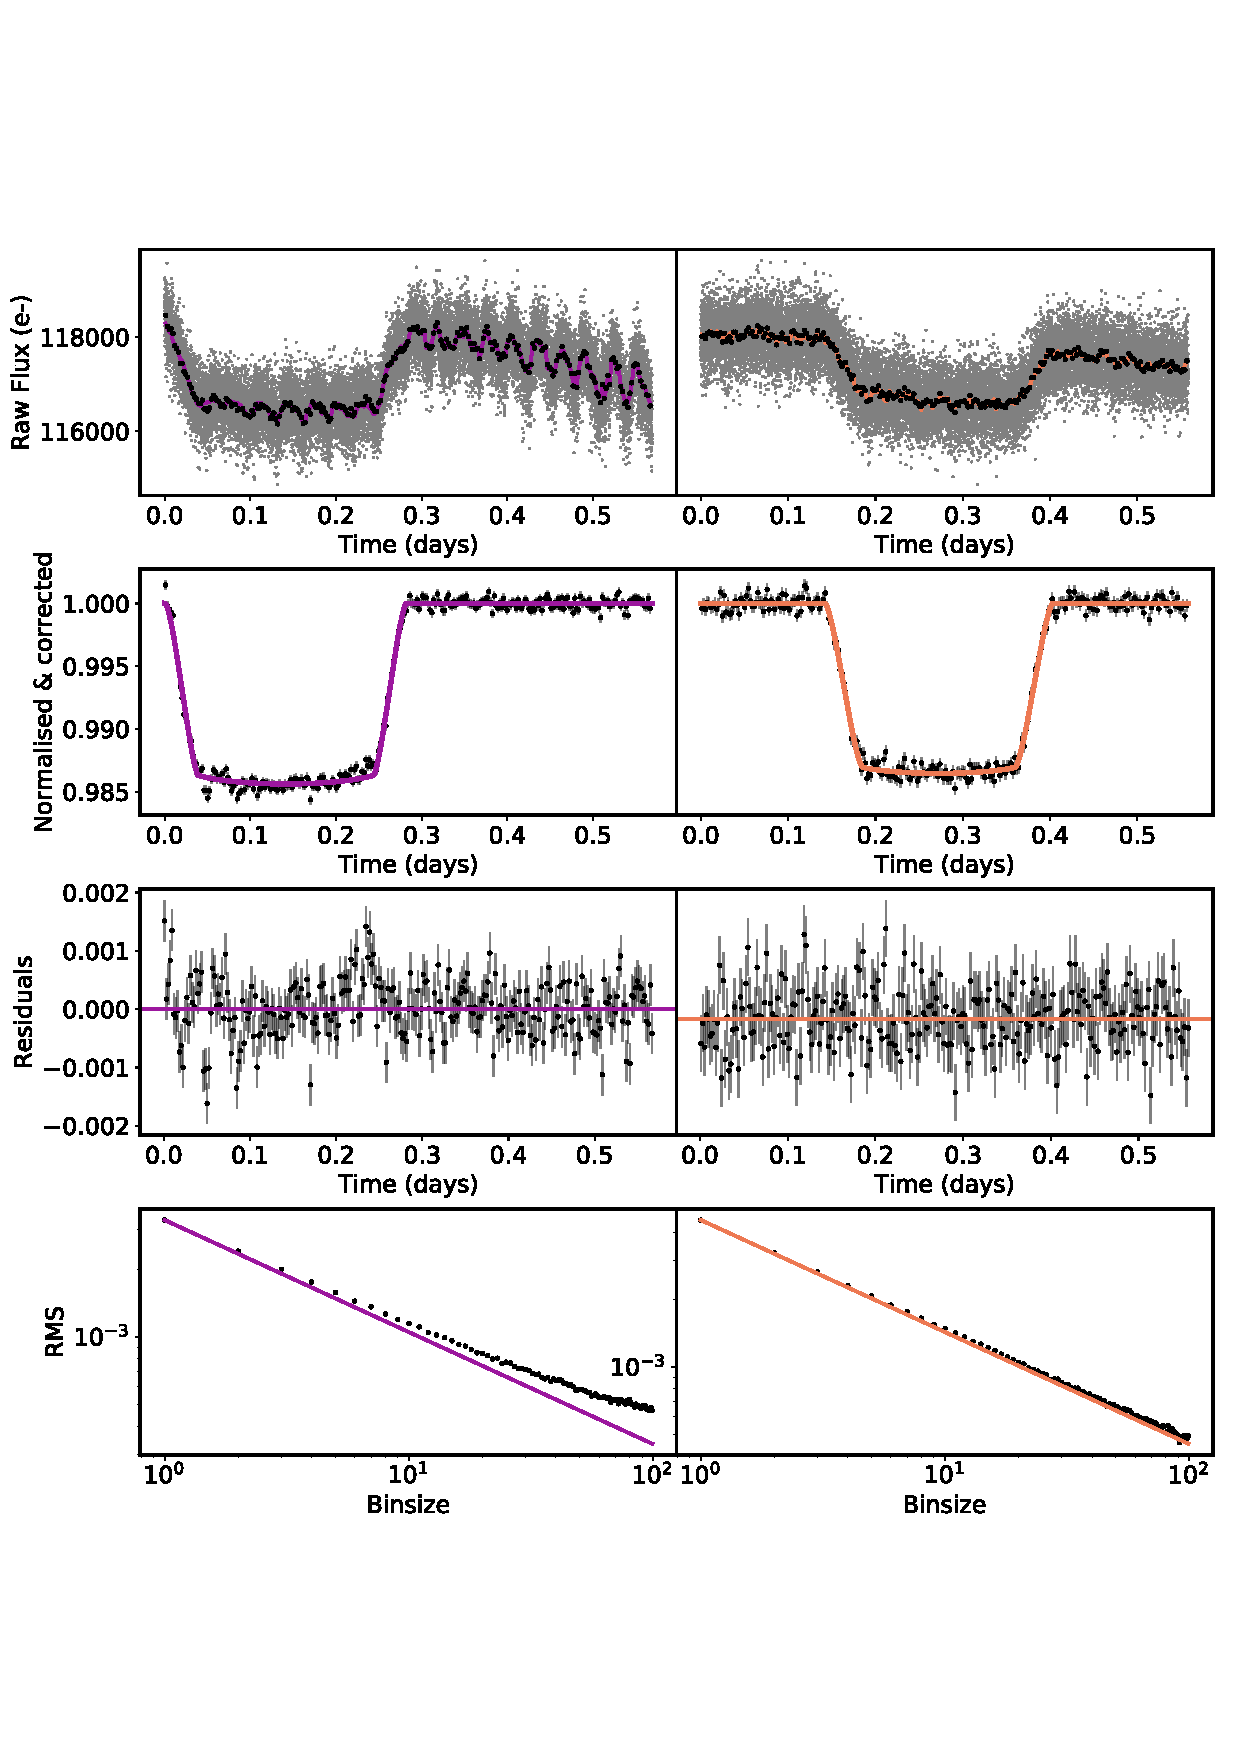
\includegraphics[width = \linewidth, trim={0 4cm 0 4cm},clip]{Kepler16b_lc.pdf}
    \caption{Left and right columns show the 3.6 and 4.5\um~ Spitzer/IRAC lightcurves for Kepler-16b respectively. Top panel: Raw flux of the transit lightcurve against time, overlaid with the best fit systematic and transit model. Second panel: Normalized and systematic corrected lightcurve, binned to roughly 5-minute intervals with the best fit transit model. Third panel: Residuals (data - model). Bottom panel: root mean squared of residuals vs bin size.}
    \label{P4:fig:k16blc}
\end{figure}

\begin{table}
    \caption{Table of the best-fit transit parameters for each of the two Spitzer/IRAC lightcurves of Kepler-16b. We show the transit depth (\rprss), the orbital distance ($a/R_s$), the inclination, and the transit time in BJD.}

    \centering
    \begin{tabular}{lll}
    \hline \hline
    Parameter & 3.6$\mu$m & 4.5$\mu$m \\
    \hline
    $(R_p/R_s)^2$ &  0.11783 $\pm$ 0.00051 & 0.11566 $\pm$ 0.00036 \\
    $a/R_s$ & 260.2776 $\pm$ 2.96 & 256.016 $\pm$ 3.44   \\
    $inc$ (deg)  & 89.89 $\pm$ 0.005 & 89.86 $\pm$ 0.005 \\
    $T_0$ (BJD) &  $2456559.0059831^{+0.0002152}_{-0.0002144}$ &  $2457010.7655917^{+0.0002496}_{-0.00025368}$ \\
    \hline
    \end{tabular}
    \label{P4:tab:spitzerresults}
\end{table}

\subsection{Comparing Kepler-16b to photodynamical model}


\begin{sidewaysfigure}
    \centering
    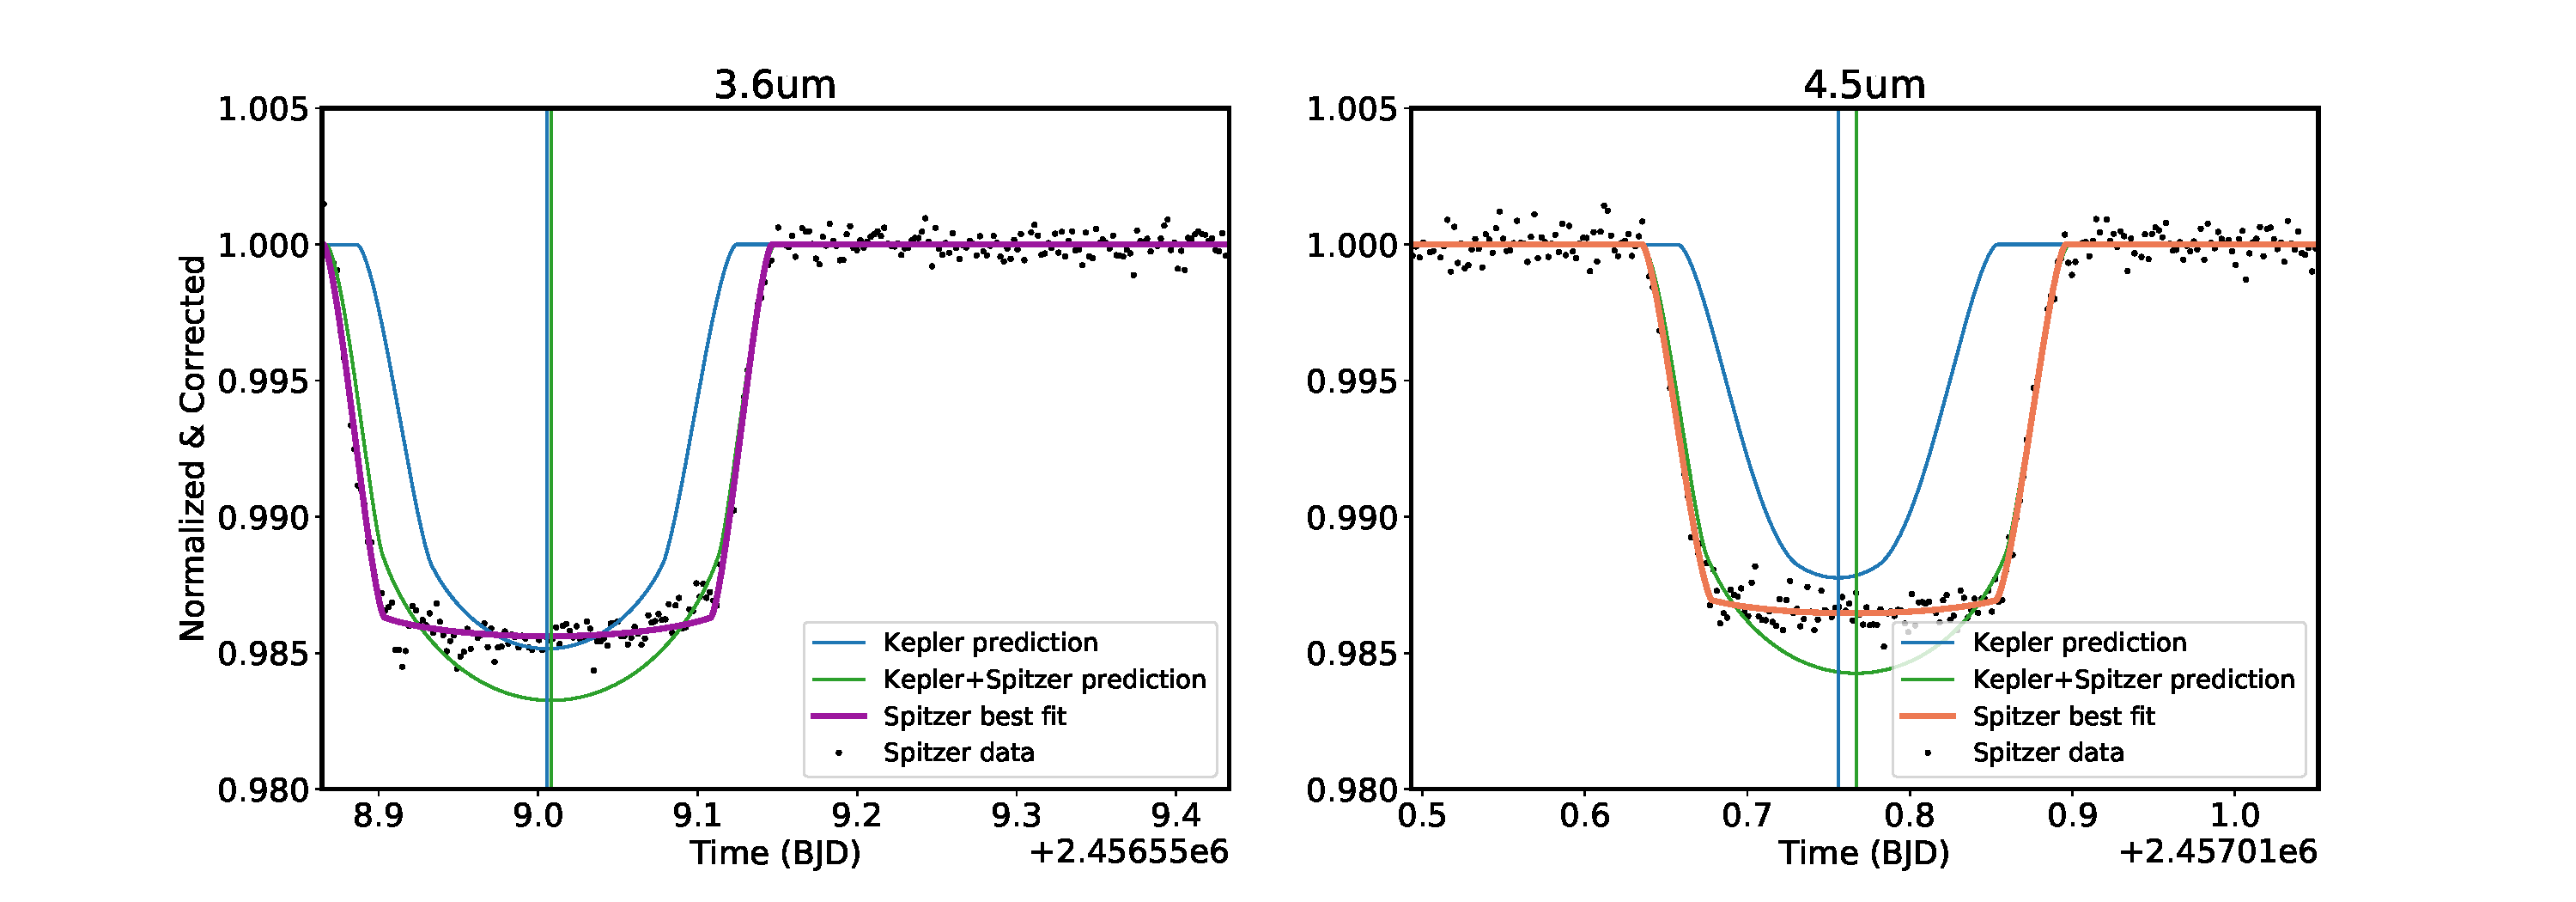
\includegraphics[trim={3cm 0 3cm 0},clip, width=\linewidth]{Kepler16b_bestfit+pred+data.pdf}
    \caption{We show the Kepler-16b transits at 3.6\um~ (left) and 4.5\um~ (right) with the photodynamical predictions. These photodynamical transit predictions are computed with Kepler transit depths and Kepler limb darkening predictions, we are interested in comparing the timing. The blue line shows the photodynamical predictions made with the Kepler data alone and propagated into the future for the Spitzer observations. The green line shows the results from the photodynamical fit with Kepler plus Spitzer data. }
    \label{P4:fig:K16_photo}
\end{sidewaysfigure}

In Figure \ref{P4:fig:K16_photo} we plot the results of the photodynamical modeling of the last two Kepler-16b transits and compare it to the Spitzer data.
We first performed the photodynamical fit with just the Kepler data and propagated the results forward in time to the Spitzer observations. These predictions are shown in blue on Figure \ref{P4:fig:K16_photo}. We found that the 3.6\um~ transit time measured with Spitzer (on 23rd September 2013) was in agreement with the Kepler predictions, with a deviation of just 1.6$\sigma$. However, there was a gap of two orbital periods until the 4.5\um~ Spitzer transit and we found that during this time the observation significantly deviated from the prediction. The 4.5\um~ transit arrived 14 minutes (37$\sigma$) early. Additionally, there is a significant deviation in the depth and duration of the transit at 4.5\um, which indicates that these transits can be used to constrain the orbital elements of the photodynamical model and the precession of the circumbinary orbit in time.

\begin{sidewaysfigure}
    \centering
    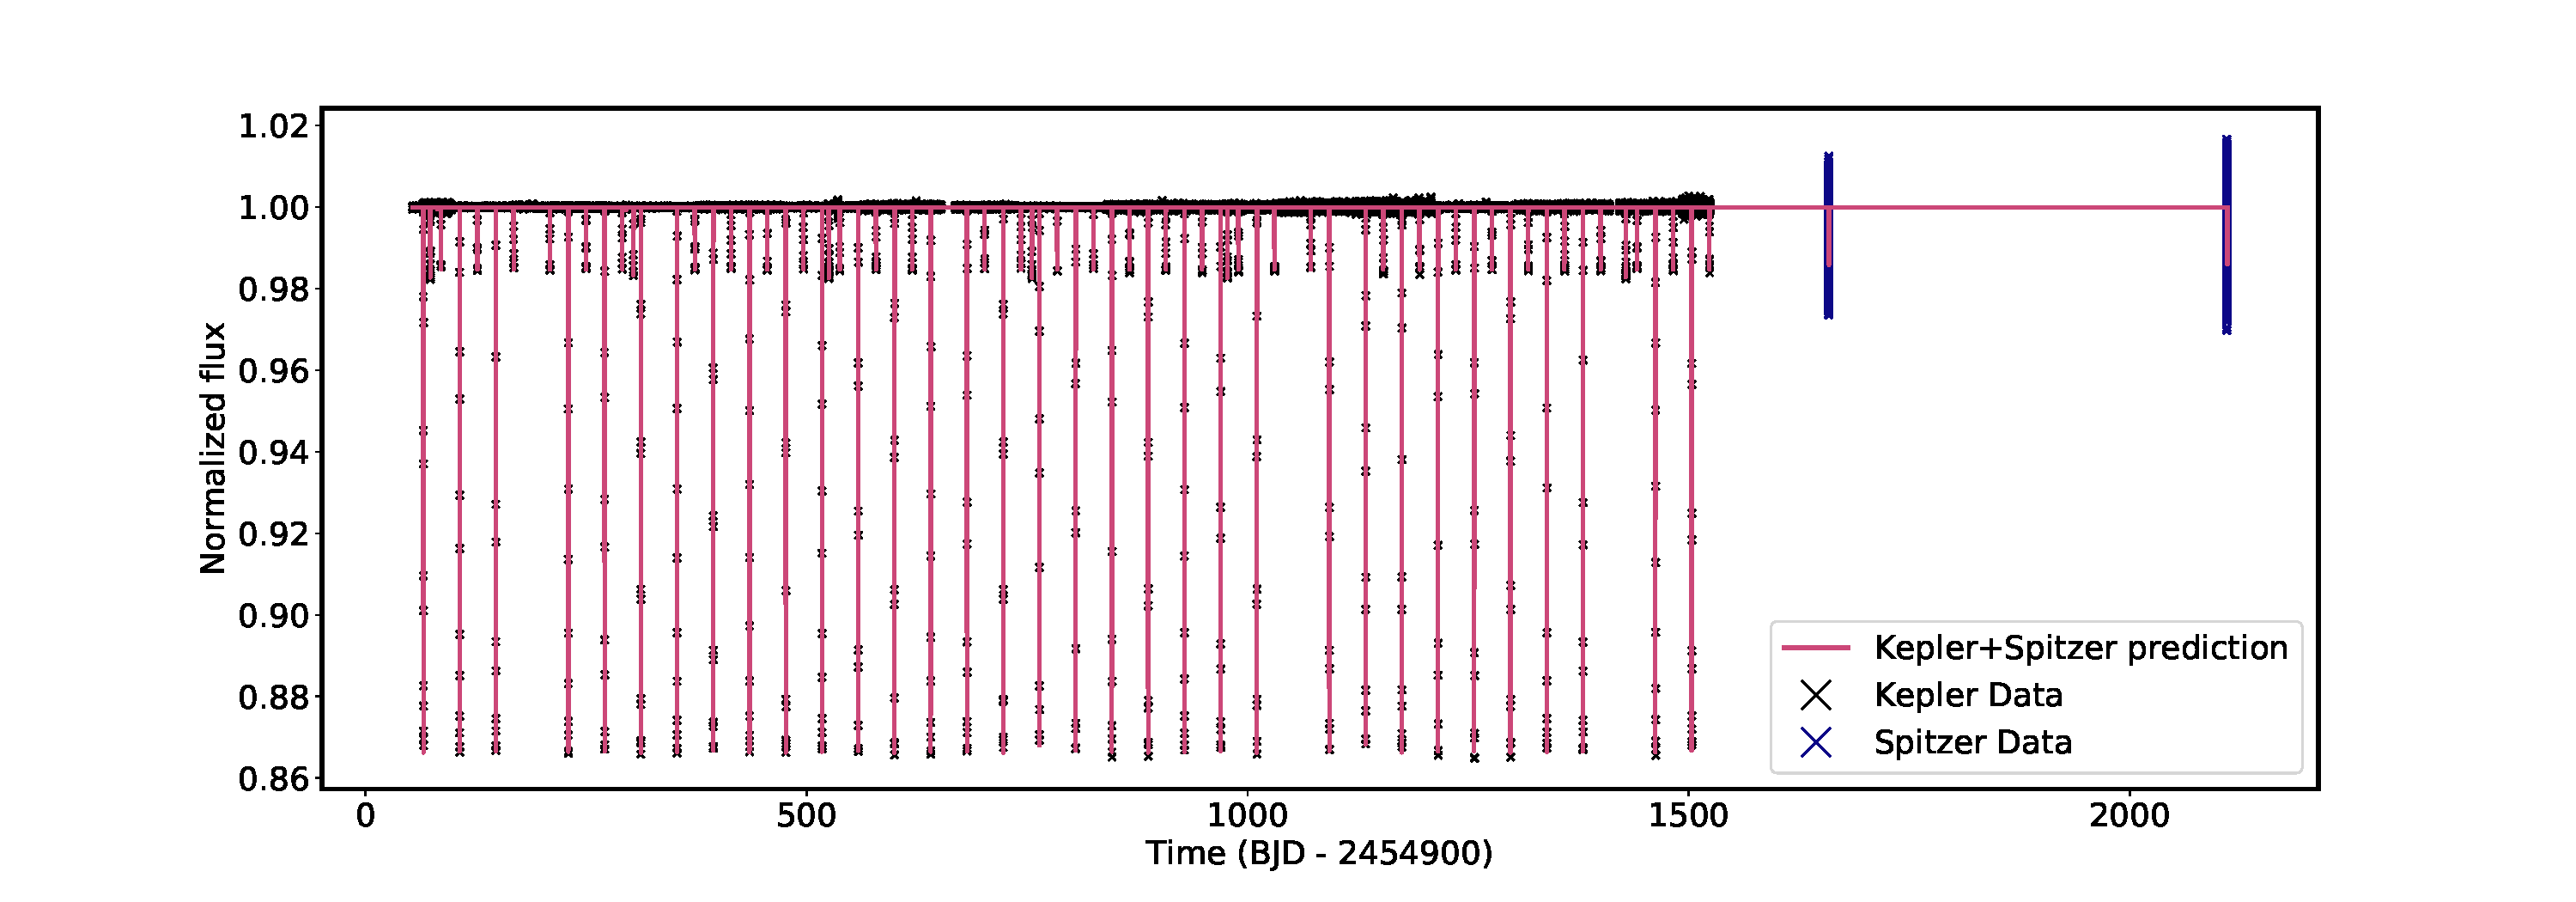
\includegraphics[trim={3cm 0 3cm 0},clip,width=\linewidth]{Kepler16b_photodynamicalmodel.pdf}
    \caption{We show the results from the photodynamical model fitting of the Kepler and Spitzer data. These photodynamical transit predictions are computed with Kepler transit depths and Kepler limb darkening predictions. The pink shows the photodynamical predictions, the black and dark blue markers show the Kepler and Spitzer data respectively.}
    \label{P4:fig:K16_model}
\end{sidewaysfigure}


In our second fit, we incorporated the Spitzer data into the fit of the photodynamical model. The resulting lightcurves are shown in green on Figure \ref{P4:fig:K16_photo}. Additionally, in Figure \ref{P4:fig:K16_model} we plot the resulting lightcurve of the photodynamical model of Kepler-16b over the entire baseline (Kepler + Spitzer). The model contains 4 types of transits/occultations in total: star B eclipsing star A, star A occulting star B, planet b transiting star A and planet b transiting star B. The two last transits in the Figure (in dark blue) show the \spitzer transits of planet b transiting star A. There are 153 days between the last \Kepler observation and the first \spitzer observation. Given that the orbital period of planet b is around 219 days, this means that the 3.6\um \spitzer lightcurve contains the next transit of planet b after the last one in the \Kepler data. Additionally, there are then two orbital periods between the 3.6 and 4.5\um Spitzer transits, which provides a significant extension to the baseline.

The best-fitting parameters for the secondary star (Kepler-16B) and the circumbinary planet (Kepler-16b) from the joint fit are given in Table \ref{P4:tab:photodynamicresults}. We also obtain a primary (Kepler-16A) mass of 0.688 $M_\odot$ and radius of 0.648 $R_\odot$.

\begin{table}  \setlength{\tabcolsep}{2pt}

    \centering

    \caption{Table of orbital elements resulting from photodynamical fit of Kepler + Spitzer data. We show the results for the secondary star (Kepler-16B) and the circumbinary planet (Kepler-16b). For each body we show the orbital period, the ephemeris ($T_0$ in BJD-2454900), eccentricity (e), inclination (i), longitude of ascending node ($\Omega$), angle of periapsis ($\omega$), mass of the planet or star ($M_p$) and the radius ratio to the primary ($R_p/R_s$).}
    \label{P4:tab:photodynamicresults}
    \begin{tabular}{lllllllll}
\hline\hline
Planet & Period  & $T_0$ & e & i & $\Omega$ & $\omega$ & $M_p$ & $R_p/R_s$    \\
       & days & BJD-2454900 & & deg & deg & deg & $M_{jup}$ & \\
\hline
Kepler-16B	& 41.0790347 & 312.1245095 & 0.163 & 90.339	& 0.0	& -96.381	& 211.990	& 0.347  \\
Kepler-16b & 228.7817675 & 530.0330639 & 0.008 & 90.029 & -0.016 & -41.445 & 0.291 & 0.118  \\
\hline
    \end{tabular}

\end{table}



\section{Discussion and Conclusion}

We have presented an analysis of 46 lightcurves using Spitzer/IRAC of 3 multi-planet systems (Kepler-9b, -9c, -18c, -18d, -32b and -32c) in an effort to constrain current TTV models. We found that the sub-array observations resulting from Spitzer entering the warm mission lead to significantly lower signal-to-noise ratios in the photometric lightcurves than predicted. These faint stars have ten times less flux than the stars of the planets studied in our previous works \citep[e.g., see][]{Baxter2021}, which results in very noisy lightcurves. Nevertheless, we performed a thorough analysis of the raw data by testing and visually inspecting all iterations of our pipeline parameters (photometry, centroiding, and background subtracting). We also tested combinations of fixed parameters from the literature, free parameters, and priors on parameters to extract the transit times from the photometric lightcurves. We present the best resulting lightcurves and the extracted transit times. Additionally, we present a version of the analysis where the transit depth is a free parameter and calculated that we do not have the precision to detect a molecular signature in the atmosphere.

We derived the transit times from Kepler data of these same planets and used an N-body model to determine the orbital elements and masses. We propagated the orbital elements forward in time to obtain posterior transit times for the times of the Spitzer transits. We compared the Kepler predictions to the Spitzer data in the hopes of constraining the TTV model. However, we found no significant deviation from the TTV predictions and the O-C plots demonstrated significant scatter. We conclude that the transits of these multi-planet systems measured with Spitzer/IRAC are consistent with but are not offering any additional constraints to current TTV models.

Additionally, we present the analysis of two Spitzer transits of the circumbinary planet Kepler-16b, one at 3.6\um and one at 4.5\um. These transits provide exquisite precision on the transit parameters. In particular, the transit times are measured to 22- and 17-second precision respectively. Using archival Kepler data, we created a photodynamical model of the system and propagated it to the time of the Spitzer observations. We found a significant deviation (37$\sigma$) between the second Spitzer transit and the predictions, suggesting that the Spitzer observations could be used to update the model and constrain the orbital elements. We then ran a DEMCMC fit of the photodynamical model with Kepler plus Spitzer data and present the updated orbital elements of the circumbinary Kepler-16 system.

\begin{subappendices}

\section{Supplementary plots}
\label{P4:app:plots}

%\section{Individual lightcurves for Kepler 9, 18 and 32 planets}

\begin{figure*}
  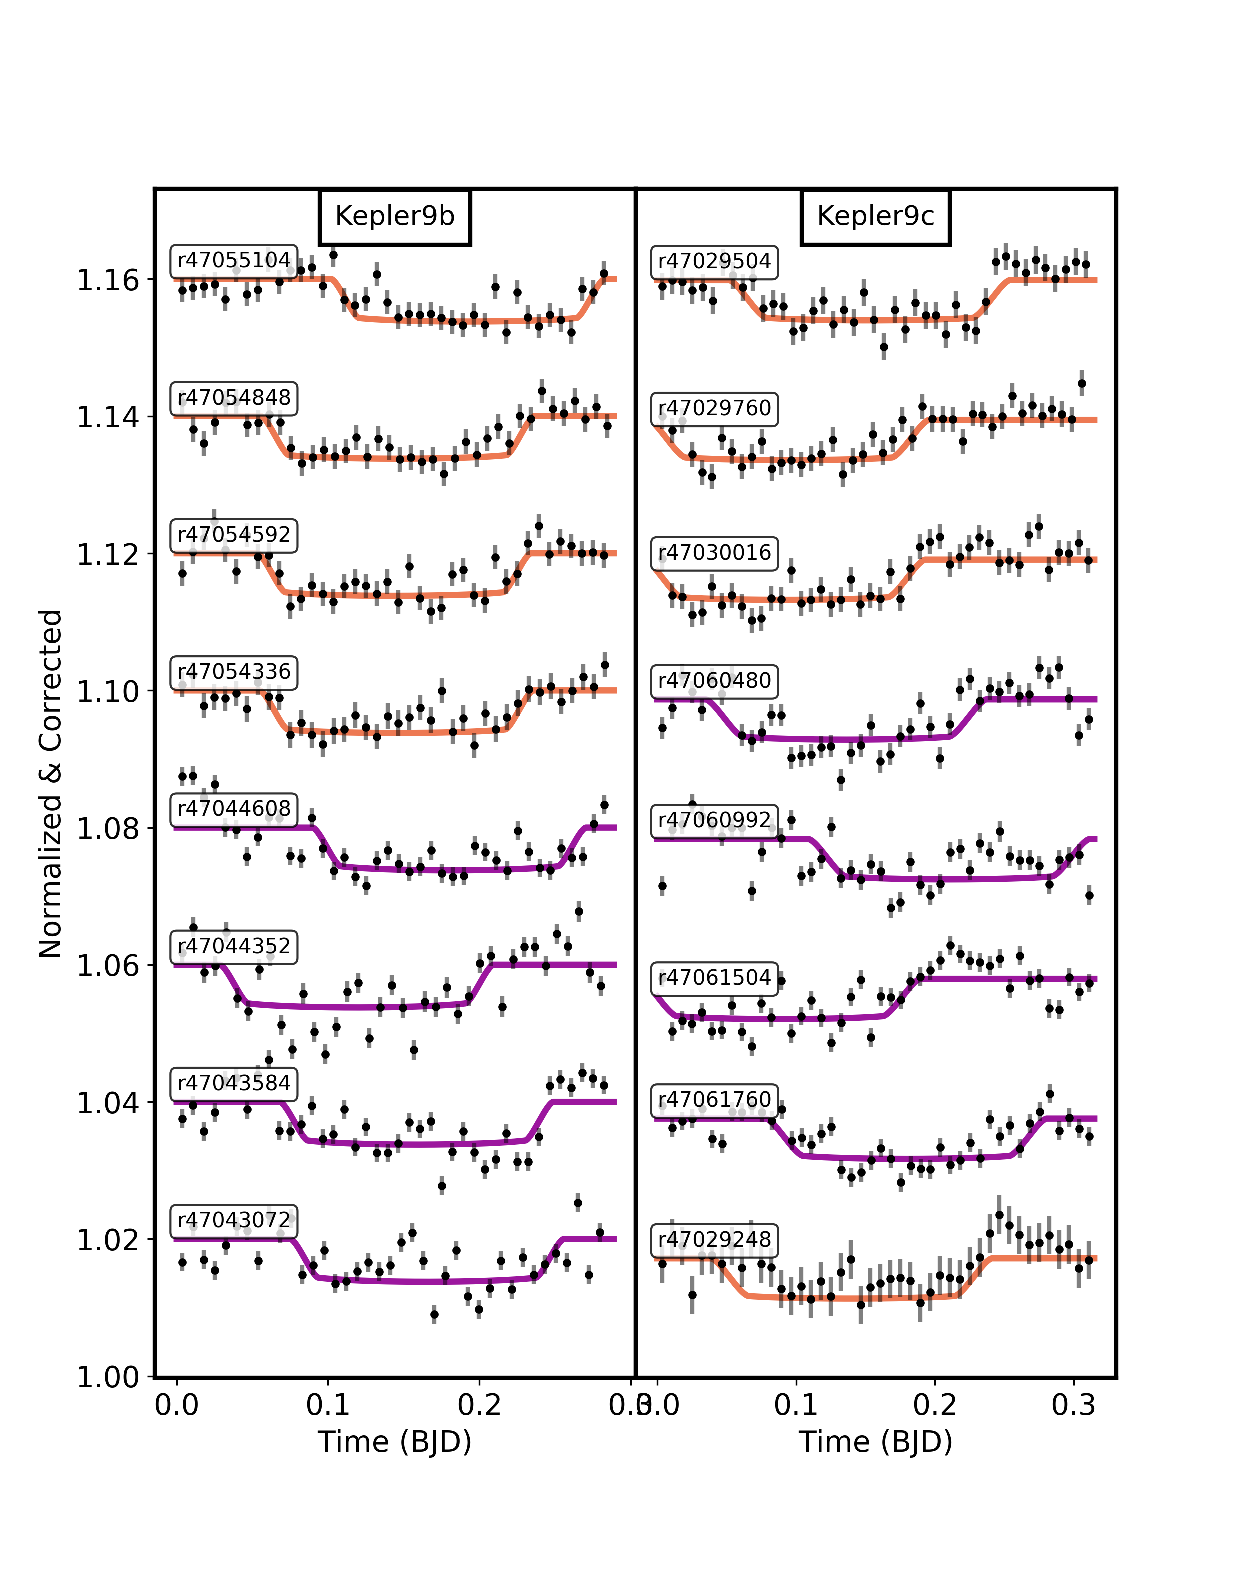
\includegraphics[trim={0 2cm 0 0},clip,width=\textwidth]{CorrectedLighctuvesPLDKepler9_circ_fixaincrp_new.pdf}
  \caption{Normalized and systematic corrected transit lightcurves for each planet in the Kepler-9 system. Left panel shows Kepler-9b and right panel shows Kepler-9c. Continuous curves show the best fit transit models, 3.6~$\mu$m in orange and 4.5~$\mu$m in purple. 1 $\sigma$ uncertainties on each photometric point are calculated from scaled photon noise. The data and these uncertainties are binned in 10 minute intervals for display purposes.}
  \label{P4:fig:normlcK9}
\end{figure*}

\addtocounter{figure}{-1}
\begin{figure*}
  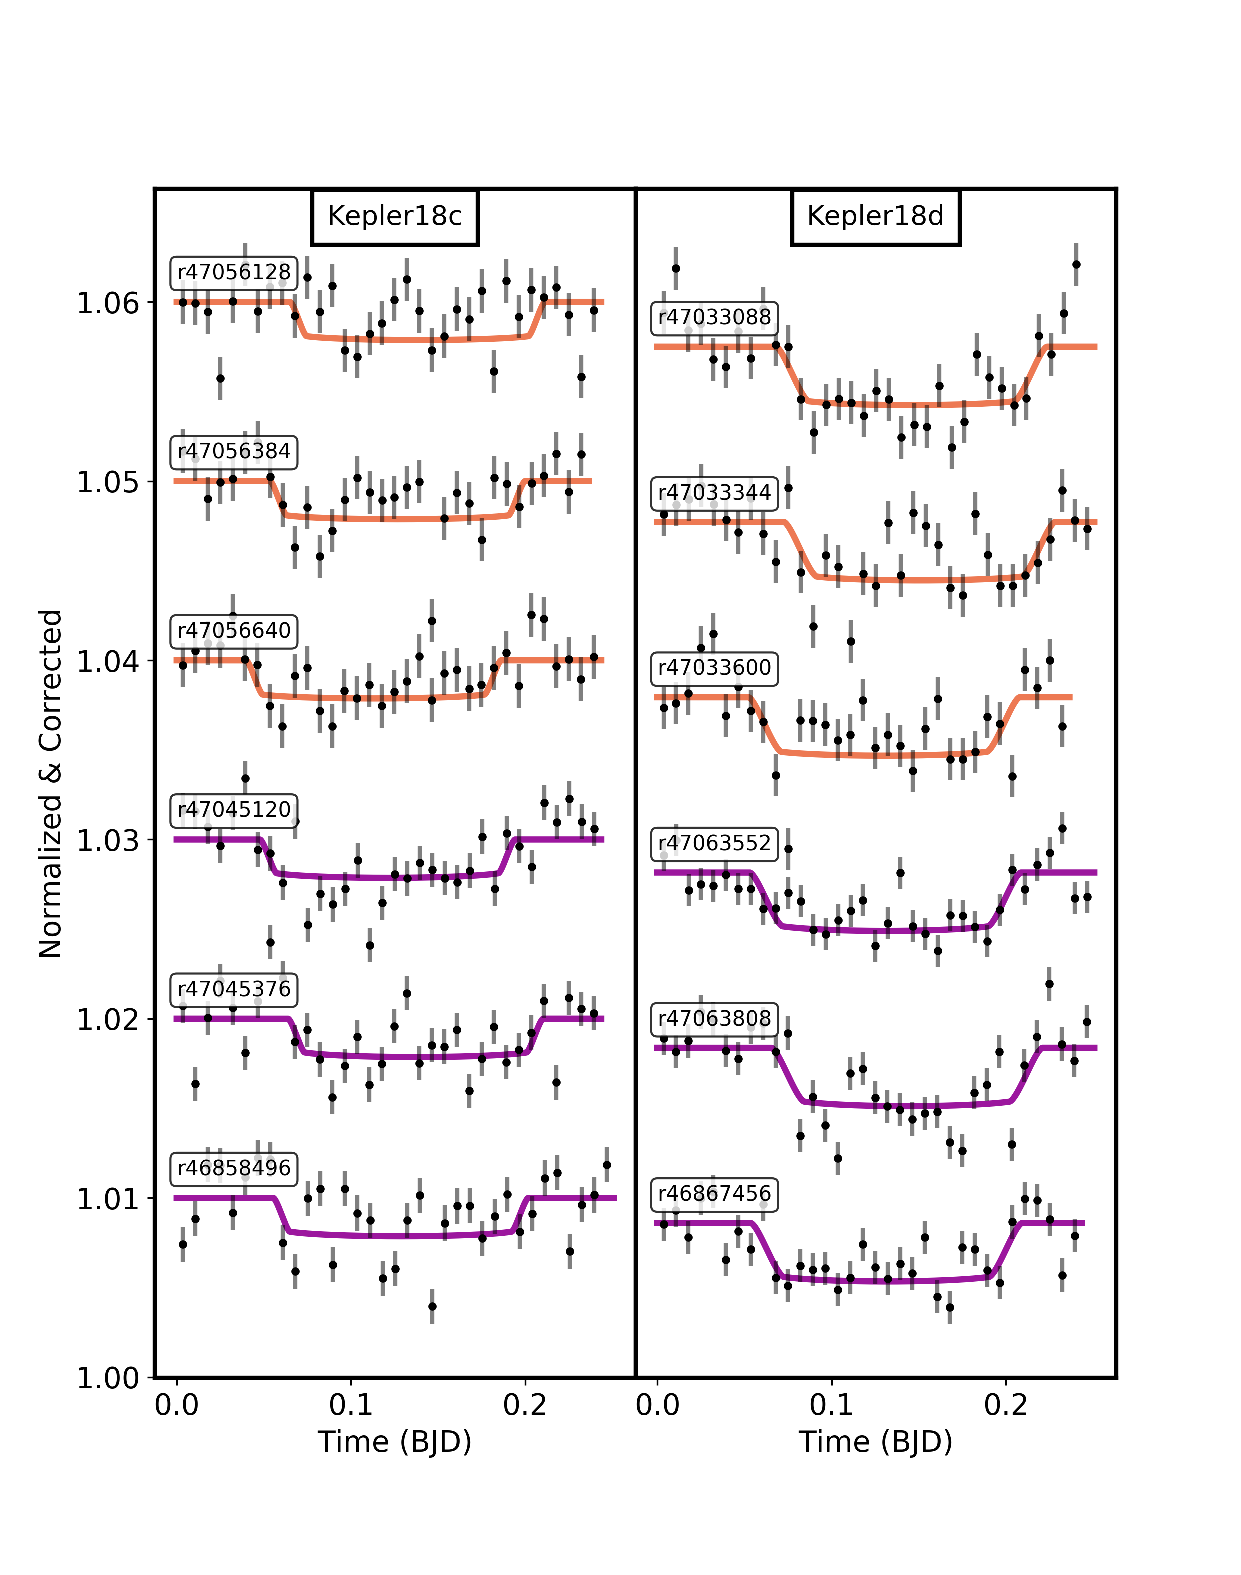
\includegraphics[trim={0 2cm 0 0},clip,width=\textwidth]{CorrectedLighctuvesPLDKepler18_circ_fixaincrp.pdf}
  \caption{Continued. Left panel shows Kepler-18c and right panel shows Kepler-18d.}
  \label{P4:fig:normlcK18}
\end{figure*}

\addtocounter{figure}{-1}
\begin{figure*}
  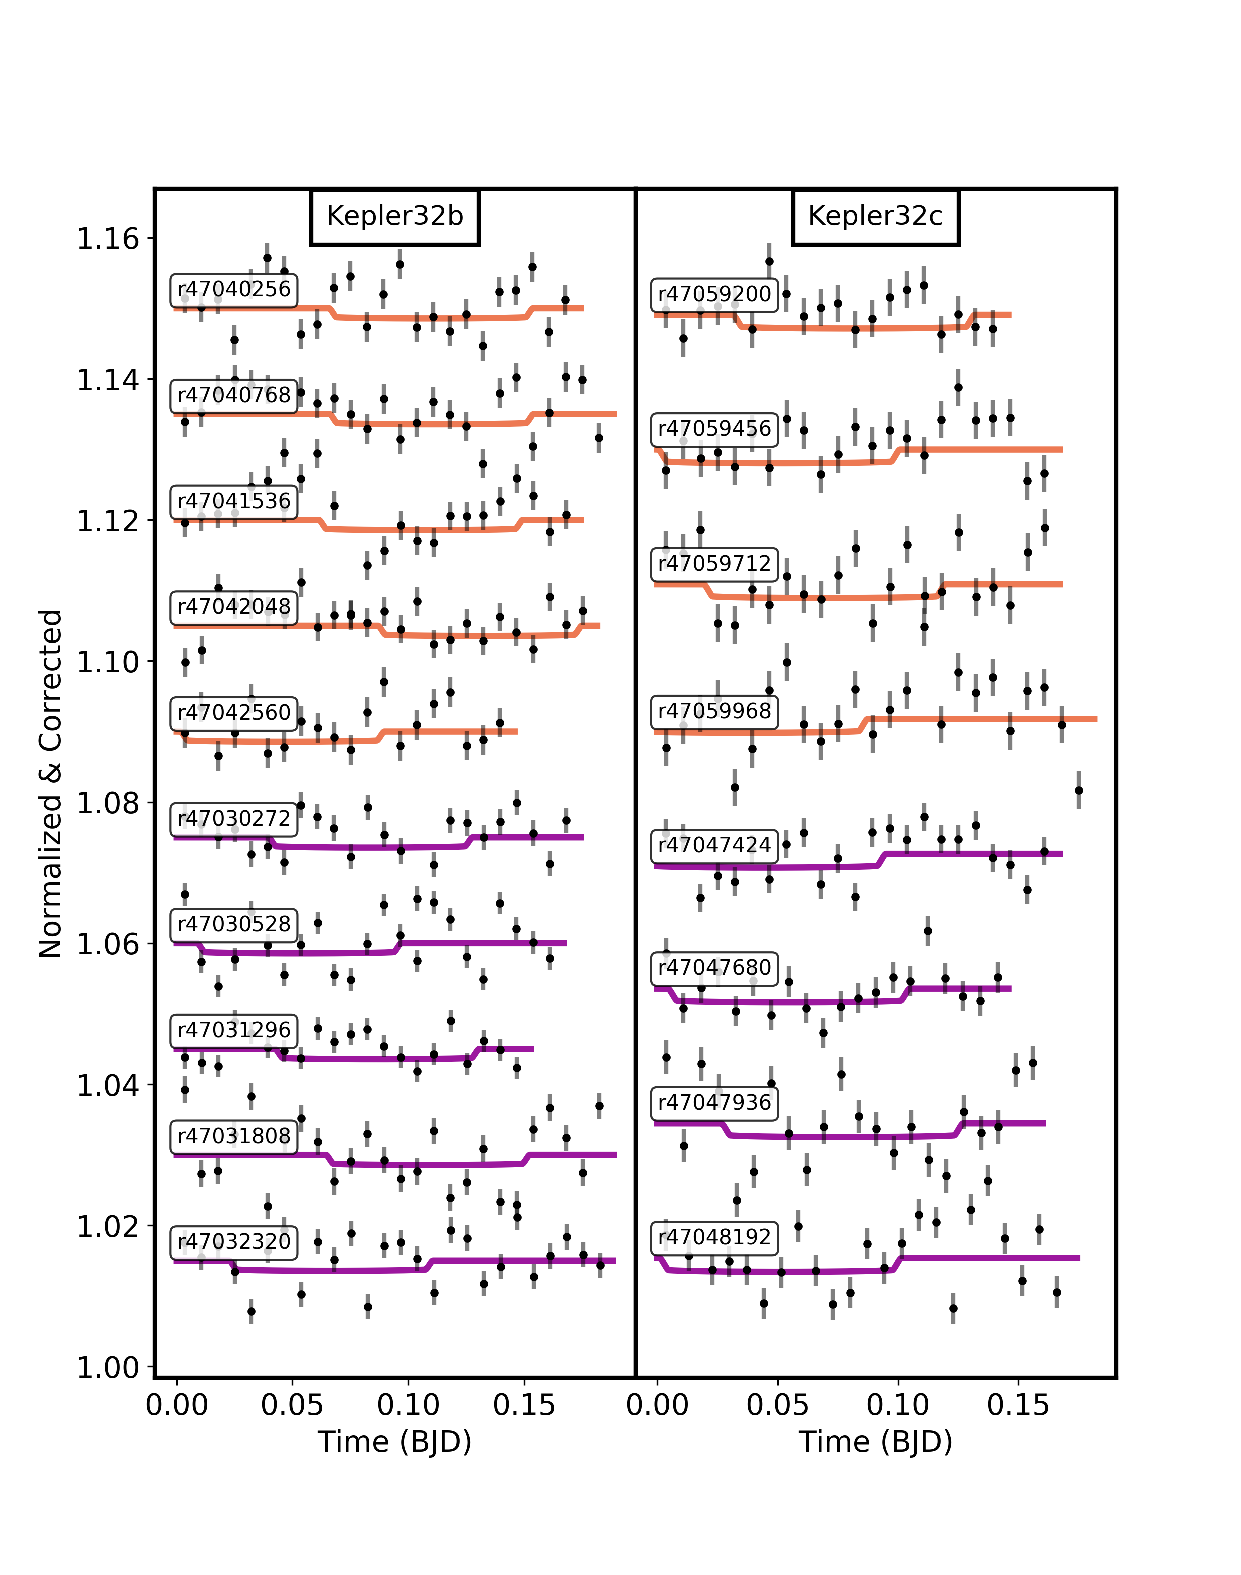
\includegraphics[trim={0 1cm 0 0},clip,width=\textwidth]{CorrectedLighctuvesPLDKepler32_circ_fixaincrp.pdf}
  \caption{Continued. Left panel shows Kepler-32b and right panel shows Kepler-32c.}
  \label{P4:fig:normlcK32}
\end{figure*}

%\section{Transit depths of multi-planet systems}

\begin{figure*}
    \centering
    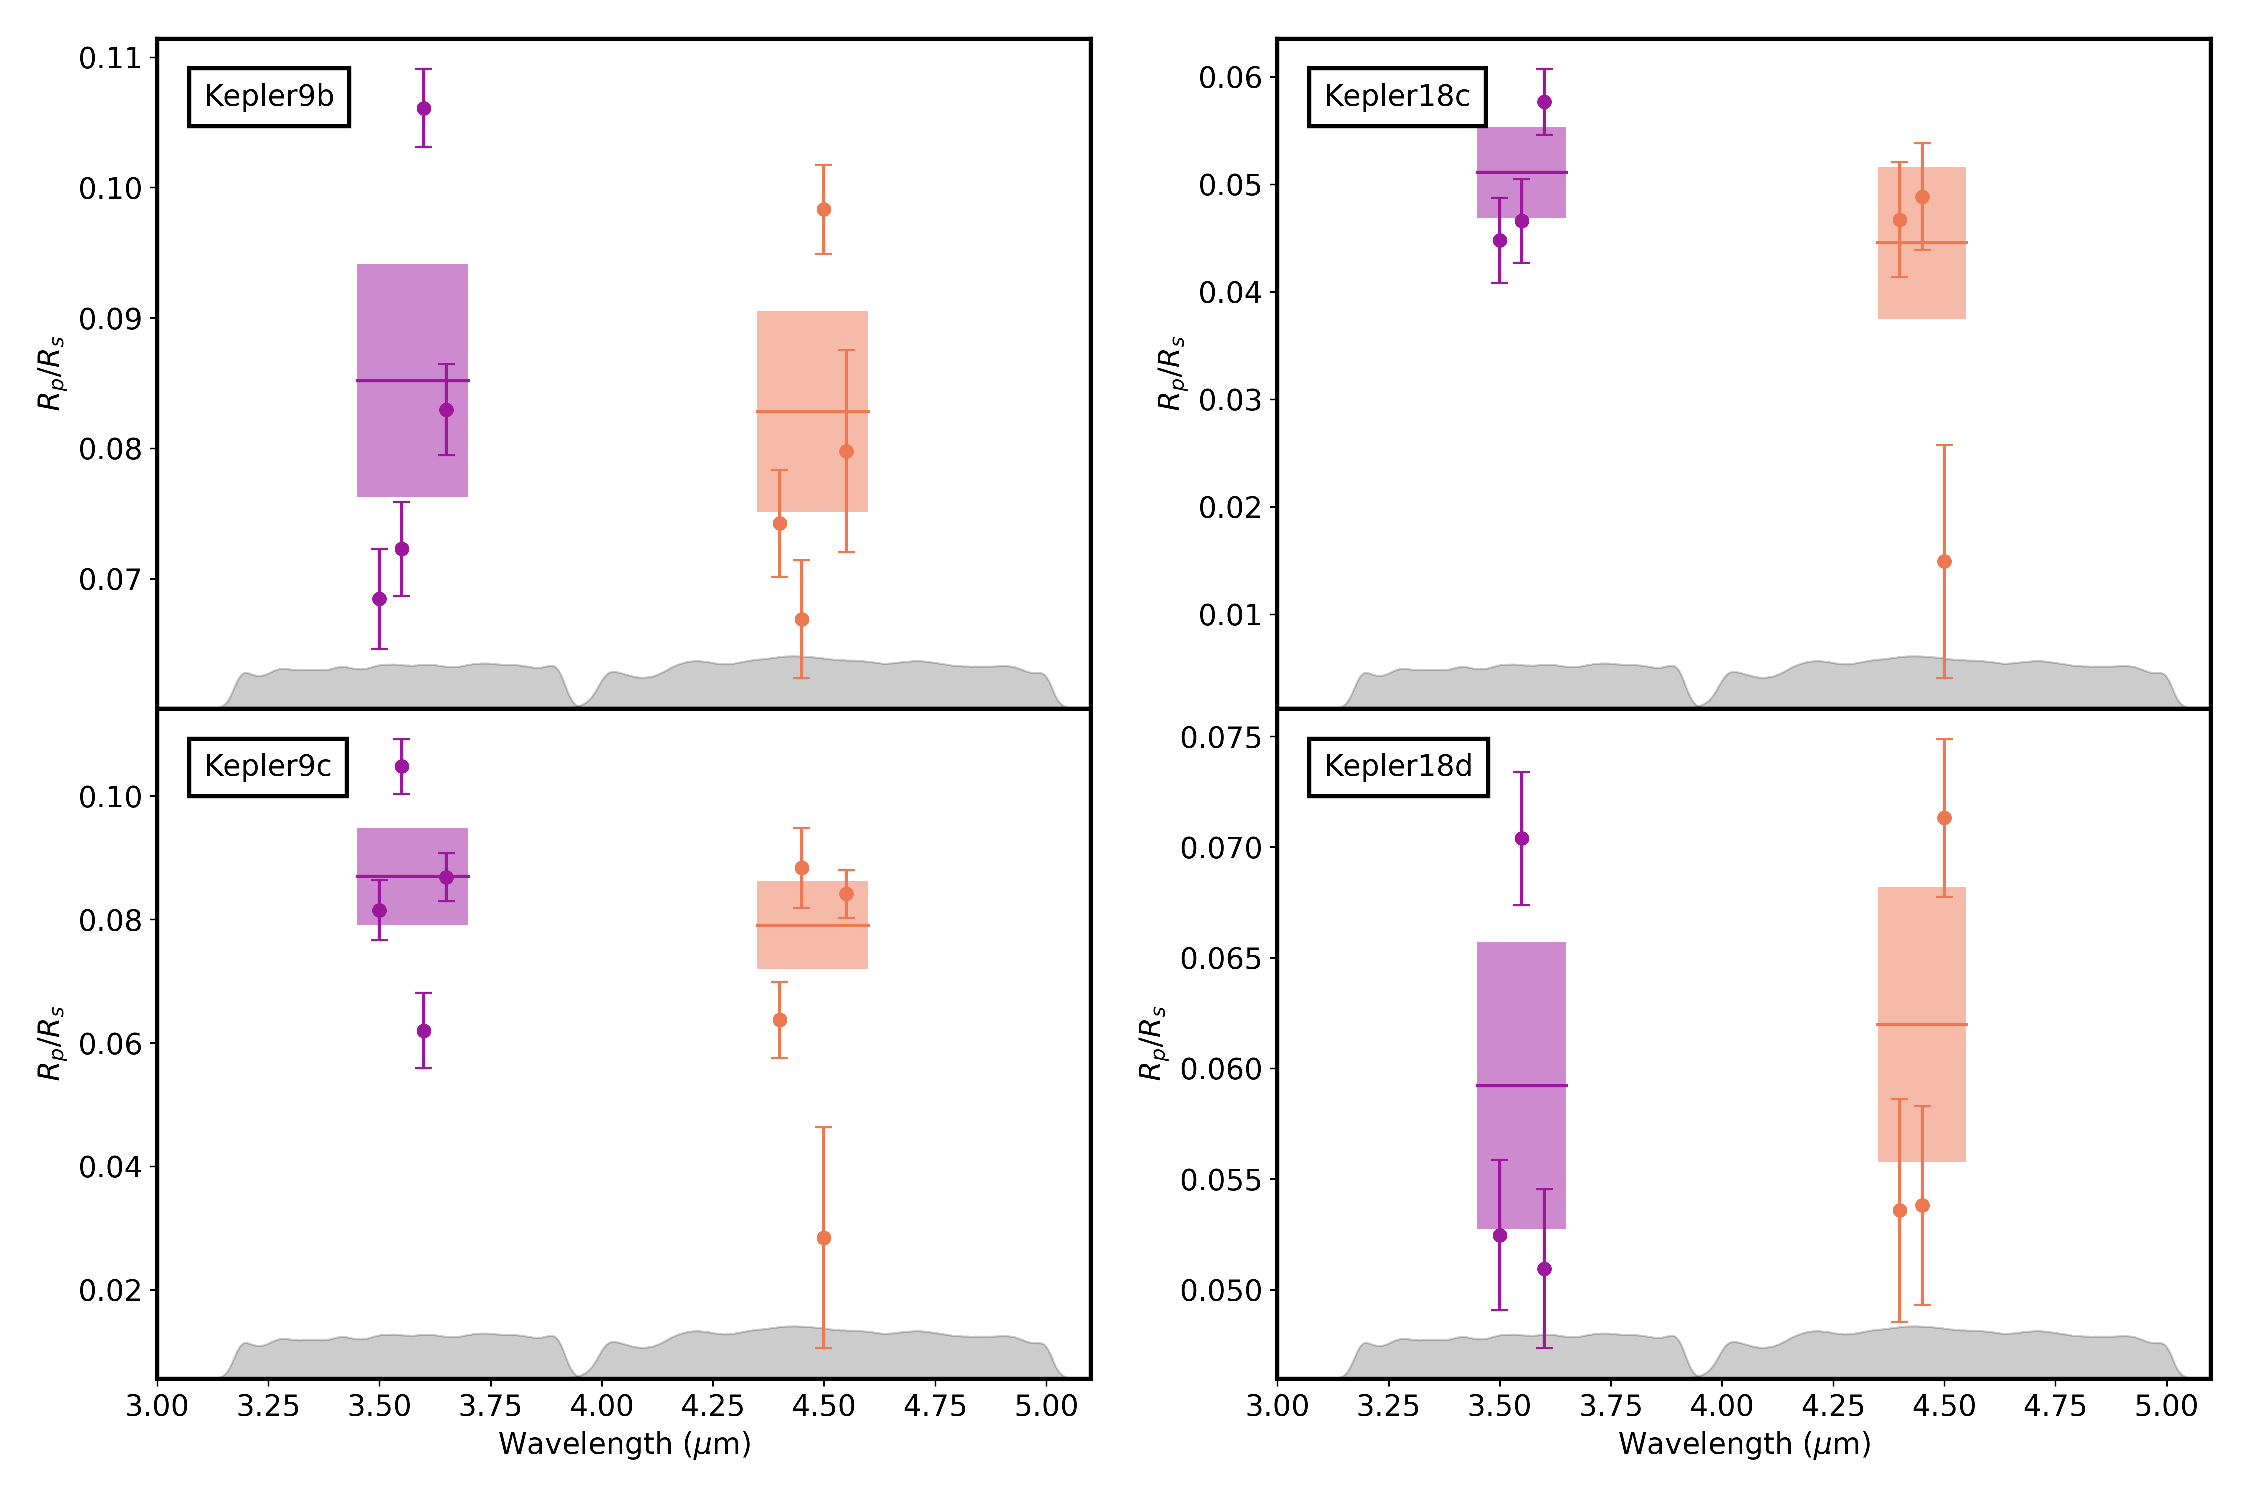
\includegraphics[width =\linewidth]{TransitDepths.pdf}
    \caption{Transit depths and their 1$\sigma$ uncertainties of each observation of Kepler-9b, Kepler-9c, Kepler-18c and Kepler-18d. Spitzer response functions are plotted in gray and the weighted mean and weighted error of the transit depths (\rprss) for each channel are shown with the colored shaded region. 3.6\um~in purple and 4.5\um~in orange.}
    \label{P4:fig:TD}
\end{figure*}

\begin{table}
  \setlength{\tabcolsep}{3pt}
    \centering
        \caption{Table of measured transit times and transit depths for Kepler-9 and Kepler-18 planets. We show the time and uncertainty in $\rm BJD_{UTC}$, the uncertainty converted to minutes and the transit depth (\rprss). }
    \begin{tabular}{llllll}
    \hline\hline
Planet & AOR & $\lambda$ &  T0 &   $\sigma_{\rm T0}$  & $(R_p/R_s)^2$ \\
& & $\mu$m & $\rm BJD_{UTC}$ & Minutes &  \\
\hline
Kepler9b &  r47043072 &     3.6 &  2.456671e+06 $\pm$ 0.003107 &    4.473655 &  0.068431 $\pm$ 0.003821 \\
Kepler9b &  r47043584 &     3.6 &  2.456632e+06 $\pm$ 0.002756 &    3.968588 &  0.072281 $\pm$ 0.003617 \\
Kepler9b &  r47044352 &     3.6 &  2.456536e+06 $\pm$ 0.001378 &    1.984667 &  0.106083 $\pm$ 0.003005 \\
Kepler9b &  r47044608 &     3.6 &  2.456478e+06 $\pm$ 0.003905 &    5.623396 &  0.082942 $\pm$ 0.003496 \\
Kepler9b &  r47054336 &     4.5 &  2.456863e+06 $\pm$ 0.003636 &    5.236191 &  0.074248 $\pm$ 0.004110 \\
Kepler9b &  r47054592 &     4.5 &  2.456651e+06 $\pm$ 0.004495 &    6.472122 &  0.066890 $\pm$ 0.004531 \\
Kepler9b &  r47054848 &     4.5 &  2.456555e+06 $\pm$ 0.001817 &    2.616881 &  0.098337 $\pm$ 0.003420 \\
Kepler9b &  r47055104 &     4.5 &  2.456517e+06 $\pm$ 0.004150 &    5.976012 &  0.079762 $\pm$ 0.007760 \\
Kepler9c &  r47029248 &     4.5 &  2.456994e+06 $\pm$ 0.004427 &    6.374814 &  0.063701 $\pm$ 0.006222 \\
Kepler9c &  r47061760 &     3.6 &  2.456294e+06 $\pm$ 0.002448 &    3.525807 &  0.081451 $\pm$ 0.004860 \\
Kepler9c &  r47061504 &     3.6 &  2.456606e+06 $\pm$ 0.002054 &    2.957437 &  0.104802 $\pm$ 0.004421 \\
Kepler9c &  r47060992 &     3.6 &  2.456839e+06 $\pm$ 0.030353 &   43.708638 &  0.061969 $\pm$ 0.006118 \\
Kepler9c &  r47060480 &     3.6 &  2.456917e+06 $\pm$ 0.002838 &    4.087393 &  0.086838 $\pm$ 0.003902 \\
Kepler9c &  r47030016 &     4.5 &  2.456567e+06 $\pm$ 0.002927 &    4.215005 &  0.088371 $\pm$ 0.006494 \\
Kepler9c &  r47029760 &     4.5 &  2.456645e+06 $\pm$ 0.069111 &   99.520470 &  0.028413 $\pm$ 0.017901 \\
Kepler9c &  r47029504 &     4.5 &  2.456878e+06 $\pm$ 0.002770 &    3.988523 &  0.084158 $\pm$ 0.003908 \\
Kepler18d &  r46867456 &     3.6 &  2.456254e+06 $\pm$ 0.003540 &    5.097910 &  0.052459 $\pm$  0.003396\\
Kepler18d &  r47063808 &     3.6 &  2.456610e+06 $\pm$ 0.001513 &    2.178499 &  0.070387 $\pm$  0.003015\\
Kepler18d &  r47063552 &     3.6 &  2.456655e+06 $\pm$ 0.003871 &    5.573921 &  0.050935 $\pm$  0.003587\\
Kepler18d &  r47033600 &     4.5 &  2.456581e+06 $\pm$ 0.005868 &    8.450013 &  0.053577 $\pm$  0.005039\\
Kepler18d &  r47033344 &     4.5 &  2.456625e+06 $\pm$ 0.002928 &    4.216482 &  0.053800 $\pm$  0.004481\\
Kepler18d &  r47033088 &     4.5 &  2.456685e+06 $\pm$ 0.002511 &    3.616499 &  0.071315 $\pm$  0.003559\\
Kepler18c &  r46858496 &     3.6 &  2.456260e+06 $\pm$ 0.005614 &    8.084660 &  0.044786 $\pm$  0.003964\\
Kepler18c &  r47045376 &     3.6 &  2.456275e+06 $\pm$ 0.005766 &    8.302904 &  0.046585 $\pm$  0.003877\\
Kepler18c &  r47045120 &     3.6 &  2.456588e+06 $\pm$ 0.003746 &    5.394609 &  0.057670 $\pm$  0.003047\\
Kepler18c &  r47056640 &     4.5 &  2.456520e+06 $\pm$ 0.004408 &    6.347335 &  0.046707 $\pm$  0.005354\\
Kepler18c &  r47056384 &     4.5 &  2.456573e+06 $\pm$ 0.004130 &    5.947279 &  0.048846 $\pm$  0.004948\\
Kepler18c &  r47056128 &     4.5 &  2.456665e+06 $\pm$ 0.064899 &   93.454854 &  0.014911 $\pm$  0.010858\\
\hline
    \end{tabular}

    \label{P4:tab:keplerTDs}
\end{table}

%\label{P4:app:K16b}

\begin{figure*}
    \centering
    \includegraphics[width = \linewidth]{K16b_corner_0.pdf}
    \caption{Corner plot of the posterior distributions resulting from the MCMC fit to the 3.6~$\mu$m Spitzer/IRAC lightcurve for Kepler-16b.}
    \label{P4:fig:K16b_corner_ch1}
\end{figure*}

\begin{figure*}
    \centering
    \includegraphics[width = \linewidth]{K16b_corner_1.pdf}
    \caption{Corner plot of the posterior distributions resulting from the MCMC fit to the 4.5~$\mu$m Spitzer/IRAC lightcurve for Kepler-16b.}
    \label{P4:fig:K16b_corner_ch2}
\end{figure*}
